%!TEX root = ../thesis.tex

\graphicspath{{Chapter4/Figures/}{Chapter4/Tables/}{Chapter4/Charts/}}

\chapter{The Impact of Team Size on Structural Metrics}
\section{Introduction} %Section - 4.1 

The first research question (RQ1) seeks to establish '\textit{the impact of development team size on the internal structural attributes of software projects and the implications on its maintainability}'. In practice this means first establishing if populations of structural metrics of software, when grouped by team size, exhibit statistically significant differences. Where such a difference is observed, the nature of that difference should be ascertained.

This chapter follows a methodical approach of initially conducting foundational work to facilitate that statistical analysis. The subsequent sub-sections articulating the analyses are of incrementally increasing complexity as outlined in Figure ~\ref{fig:ChapterOverview}. Section 4.2 is titled 'Data Mining' which details efforts to extract a data sample from the broader forge and to mine the sample for structural metrics. Section 4.3 covers an initial 'Exploratory Data Analysis': efforts to understand the underlying trends in the mined data from a one-dimensional perspective in addition to the distribution and correlations within. Section 4.4 documents an initial, 'Univariate Analysis' to establish a relationship between team size and structural metrics - simplistic as the confounding impact of revisions (potentially a proxy to functional complexity) means that this analysis will not yield clear or reliable results but will serve to establish the foundation on which the further analysis will take place. These confounding factors will be the subject of Section 4.5 which factors in the impact of revisions to observe the impact of the development team size, alone, on structural metrics. In Section 4.6 the results are presented in the context of two individual projects and qualitative code-level observations are made to highlight the reasons that drive the quantitative forge-level observations. Finally Section 4.7 provides a summary of the results and relates the observed relationship between team factors and CK metrics to the likely impact on maintainability. Figure ~\ref{fig:MiningToolchain} highlights the aspects of the toolchain that will be subject to further discussion in this chapter.

\begin{landscape}
\begin{figure}[htbp!] 
\centering    
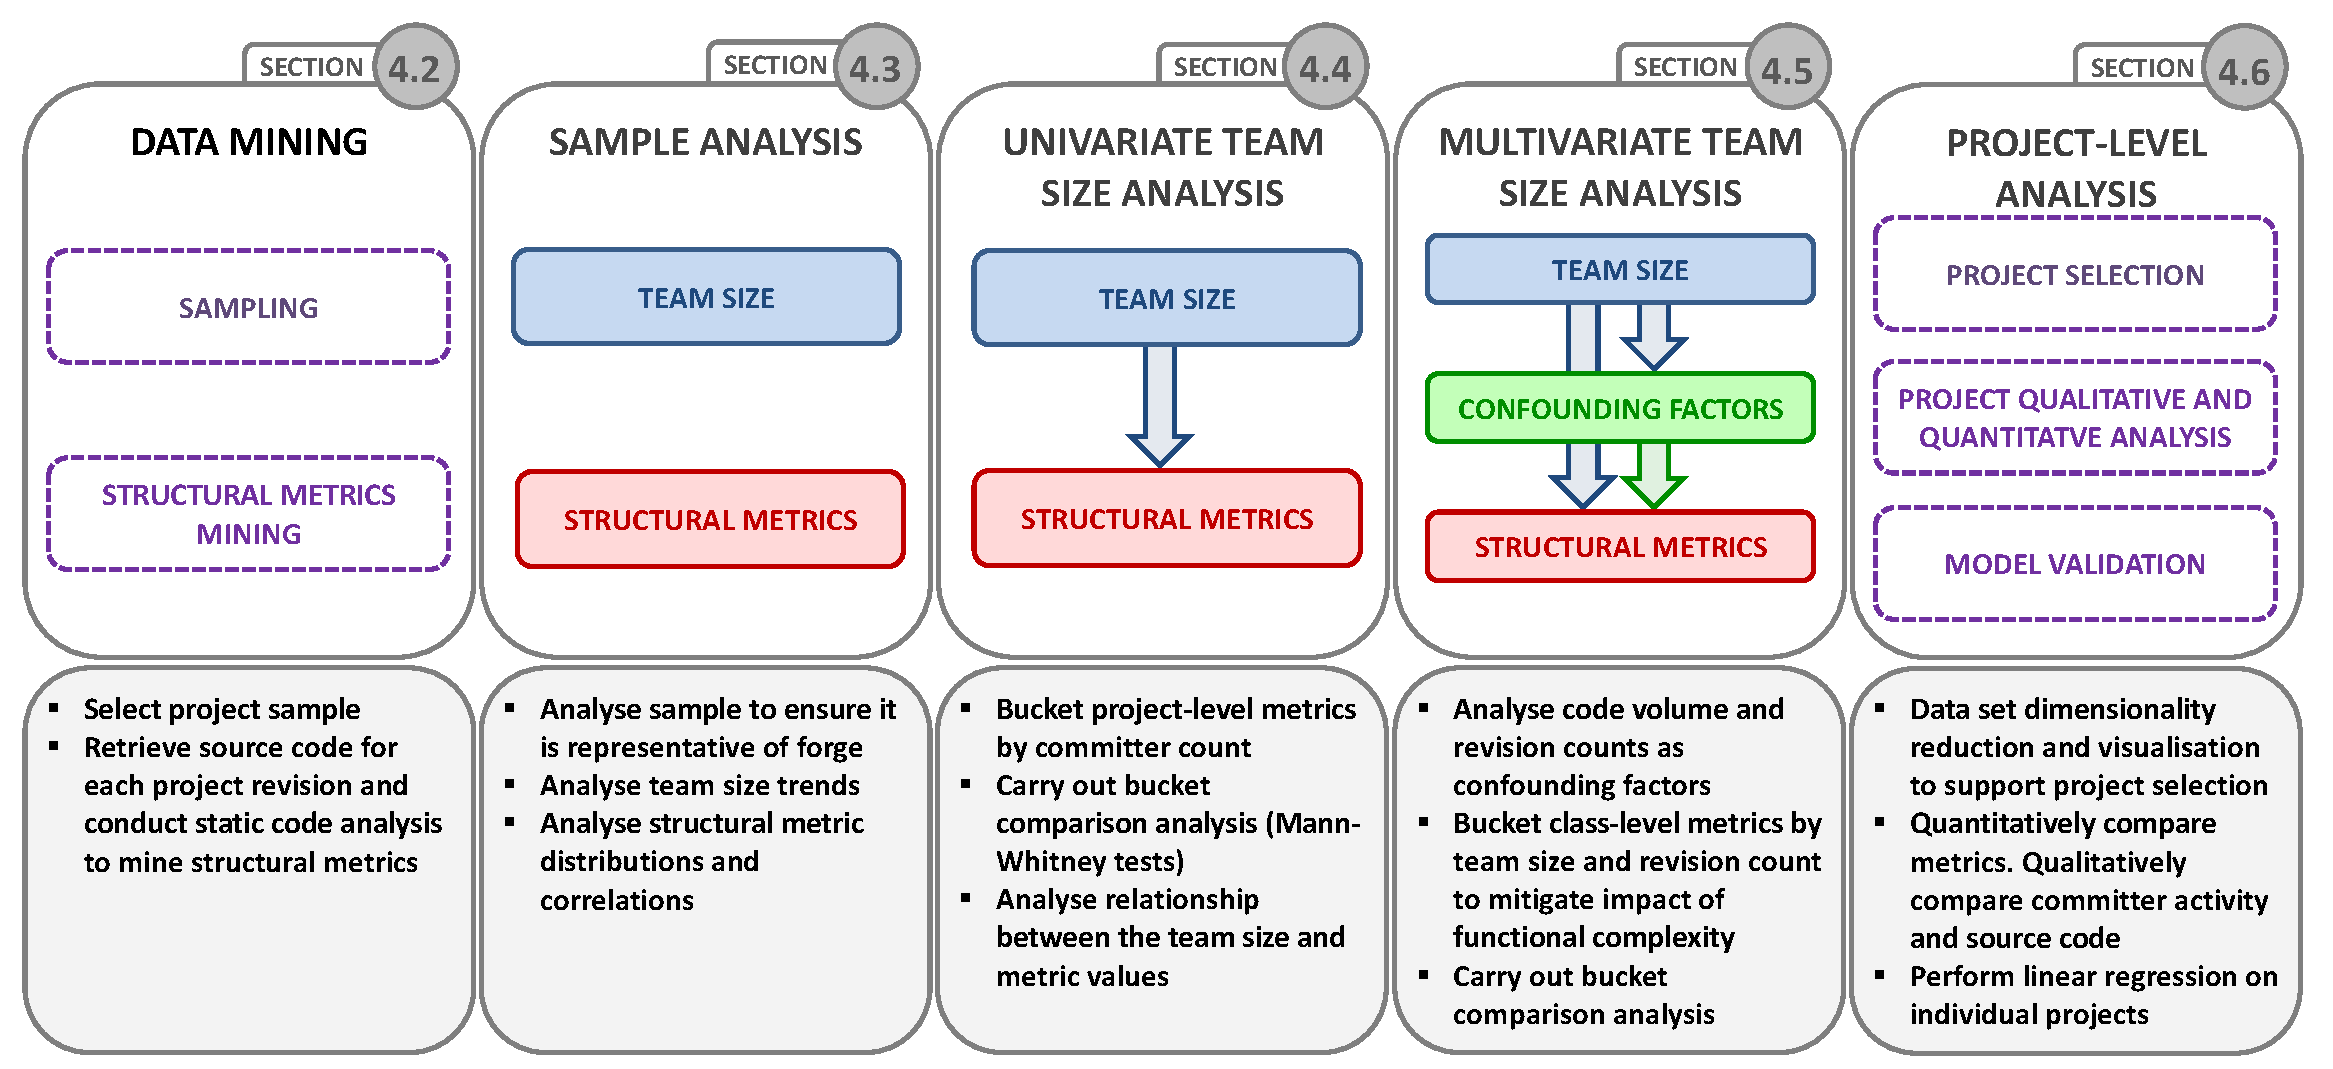
\includegraphics[width=1.4\textwidth]{ChapterOverview.pdf}
\caption{Chapter 4 outline providing an overview of the contents of each section.}
\label{fig:ChapterOverview}
\end{figure}
\end{landscape}

\begin{figure}[htbp!] 
\centering    
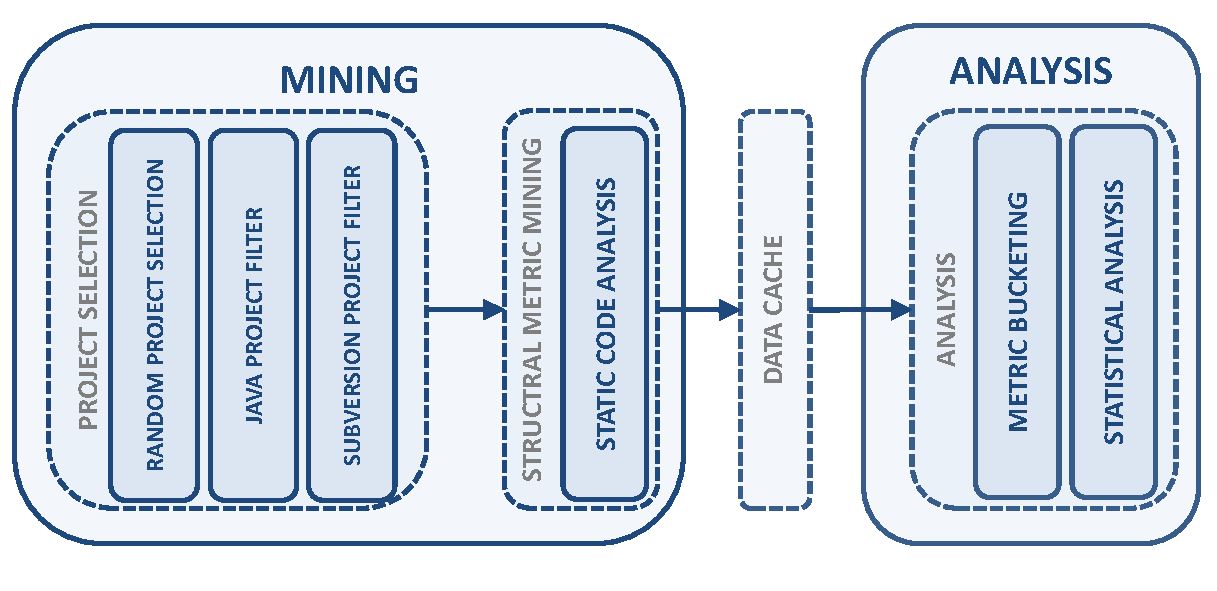
\includegraphics[width=1.0\textwidth]{MiningToolchain.pdf}
\caption[Some aspects of the toolchain pertinent to team size analysis.]{Some aspects of the toolchain pertinent to team size analysis. Project Selection and Structural Metric Mining are both the subject of discussion in section 4.2. Analysis is the subject of the remainder of the chapter.}
\label{fig:MiningToolchain}
\end{figure}
 

\section{Data Mining} %Section - 4.2
When analysing basic committer activity within a forge it is possible to learn a substantial amount through mining the revision logs across all the repositories within the forge. Although requiring significant processing, given modest resources it is computationally feasible to mine the revision history of all projects in a forge made of up several hundred thousand repositories. It is necessary to mine the entire forge when conducting network analysis (as discussed in detail in the next chapter). This, however, is not the case when conducting the detailed structural metric based analysis contained within this chapter. To mine structural metrics necessitates network, processor and storage intensive processes to execute the retrieval and static analysis of the source code at each revision for each project studied. As described in section 3.3.8 in the previous chapter this is still a very resource intensive task and it is not practical or necessary to run this type of analysis across the entirety of the forge. For the purposes of this research it is most appropriate to restrict this type of in-depth analysis to random sample of projects. 

With this context in mind, this section covers two key aspects of the data mining approach that are foundational to the team size analysis: Project Selection and Structural Metric Mining. 

\subsection{Sampling}
The project selection component was outlined in section 3.3.6 of the previous chapter and is a Java component taking, as its input, flat files made available by FLOSSmole providing a full listing of all projects hosted by GoogleCode. Its first responsibility is to identify, within this population, a sample of projects programmed in Java. As discussed earlier, Java was chosen as it increases relevance to the academic and practitioner community and restricting to projects of a single language greatly simplifies the data mining by not requiring support for static code analysis across multiple languages. While restricting the analysis to a single language aids practicality, it also presents a threat to validity when generalising the applicability of any results to projects in any other language, as was highlighted in early research \citep{basili1996validation}. While some similarities carry across object-oriented languages, earlier work has highlighted some of the structural differences between Java and C++ projects \citep{subramanyam2003empirical, english2009exploring} finding that Java lends itself to greater maintainability. These threats to validity are the subject of further discussion in Chapter 6.

While creating projects in GoogleCode the project administrator can associate 'tags' with the project. This is essentially meta-data enabling the categorisation of projects for the purposes of searching or browsing projects. FlossMole provides this meta-data in flat file format. Analysis of this meta-data shows that 204,918 projects (87\%) have at least one tag and on average each project has 4 tags defined. Given that tags are free text, there are a large number of unique tags (145,600). The top 250 most frequent tags were extracted and manually categorised accordingly. The relative occurrences of each category was then calculated on the basis of the 250 most frequent tags and depicted in Figure ~\ref{fig:ProjectCategorisation}. 

The results in Figure ~\ref{fig:ProjectCategorisation} demonstrate that tagging projects by programming language is fairly common. It follows that identifying a substantial set of Java projects is achievable through tag analysis alone. Table ~\ref{tab:GoogleCodeLanguage} shows Java as the most popular language tag associated with 22,594 projects (making it also the most popular tag in any category). This set of projects is considered the \textit{population}.

GoogleCode allowed project administrators to choose from among three available version control systems - Subversion, GIT, and Mercurial - on which to host their source code. Each of these necessitate a different mechanism to mining data. In the case of Subversion and GIT, the revision history can be directly queried (albeit through different syntax and requiring individual log parsers) while in the case of Mercurial it is necessary to clone the repository before retrieving the history - an altogether slower process. As this research is concerned with building a toolchain that can efficiently mine data from each repository type, it is necessary to understand the distribution of projects across types. Table ~\ref{tab:GoogleCodeVCS} shows that Subversion was overwhelmingly the most popular repository type. This reflects the relative popularity of these version control systems at this point in time as GIT was later to see greater adoption in the industry, eventually becoming the most popular VCS by web searches according to Google Trends \citep{rhodecode}. De Alwis and Sillito attribute this transition to the decentralised nature of GIT which allows enhanced developer access, greater support for experimental changes and improved workflows around branching and merging \citep{de2009software}. While the revision history mining effort spans all projects (necessary for comprehensive network analysis in the coming chapter), the static code analysis effort is simplified by exclusively selecting Subversion projects to mine for structural metrics.

\begin{figure}[htbp!] 
\centering    
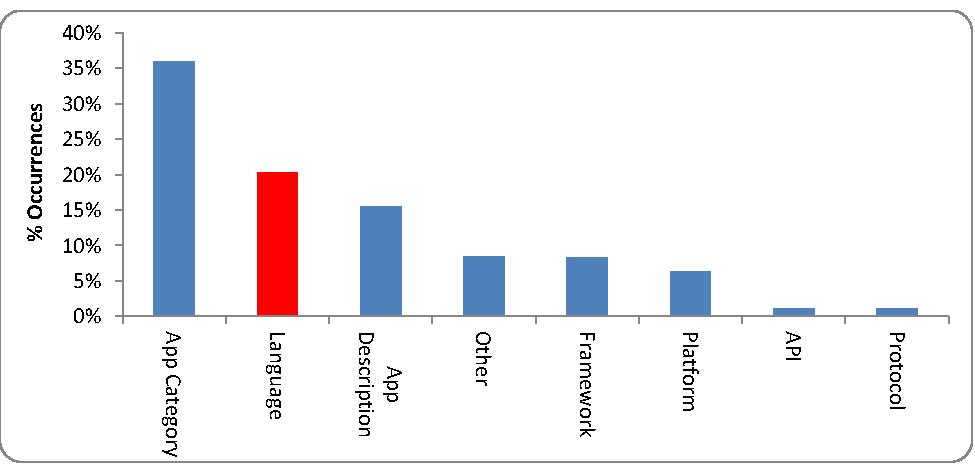
\includegraphics[width=1.0\textwidth]{ProjectCategorisation.pdf}
\caption{A representation of the categorisation of tags and their relative occurrences across the forge}
\label{fig:ProjectCategorisation}
\end{figure}

\begin{table}
\centering 
\captionof{table}{The top 5 tags within the language category showing the 'Java' tag the most popular of all.}
\begin{tabular}
 \centering 
 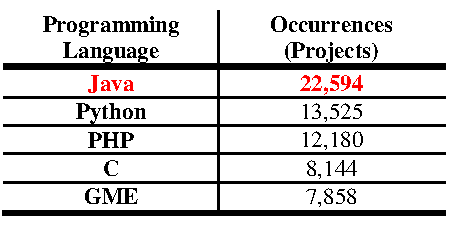
\includegraphics{GoogleCodeLanguage.pdf}
 \label{tab:GoogleCodeLanguage}
\end{tabular}
\end{table}

A \textit{sample} is extracted from the \textit{population} of 22,594 projects by iteratively invoking a simple pseudorandom function (the 'random' method in the Java Utils API which has an approximately uniform distribution) to select a number between 0-1 to be multiplied by the total number of projects available until the sample is extracted of an appropriate size. The selection algorithm discards from consideration any projects with no revision history as they represent projects which never saw committer activity beyond initial project creation and therefore have no relevance to this study. With a confidence level of 99\% and a confidence interval of 5\%, a minimum sample size of 646 was calculated. The actual sample size used was arbitrarily higher than the minimum sample size at 658 projects. 

Once the sample projects are selected, a utility in the toolchain allows for the automated parsing of the repository URL from the relevant project's page on the GoogleCode website. The project list with the associated URLs are then consolidated in a single file output which is used to drive the metric mining process.

\begin{table}
\centering 
\captionof{table}{The repository counts for each version control system across the forge.}
\begin{tabular}
 \centering 
 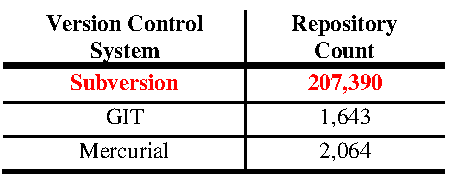
\includegraphics{GoogleCodeVCS.pdf}
 \label{tab:GoogleCodeVCS}
\end{tabular}
\end{table}


\subsection{Structural Metrics Mining}
The broad approach to mining project repositories for structural metrics is documented in section 3.3.6 of the previous chapter. This section builds upon that foundation to detail the aspects of mining that are specific to the particular analysis that forms the latter half of this chapter. For the initial univariate analysis, static code analysis is conducted on the latest version of the code of all selected projects within the sample. However, the later multivariate analysis, as will be covered in section 4.5, the identification of revision counts as a confounding factor will necessitate the analysis of every revision of each project and subsequently the static code analysis to mine for structural metrics - again for each revision. This creates a requirement to store structural metrics for each Java class file in each project for every revision of that project. Given that there can be hundreds of class files and thousands of revisions, this is a fairly large data set. In order to be able to query this data effectively there is a reliance on the database model documented in Figure ~\ref{fig:Schema}. This is in contrast to the univariate analysis where only a single set of structural metrics is captured for the entire project. Figure ~\ref{fig:AnalysisDataSets} illustrates the difference in these two approaches. On the left, there are three revisions and three classes: class A being revised three times and class C revised just once. On the right the contrast is shown between the univariate analysis (where only the final revision is considered) and the multivariate analysis (where all three revisions are considered).

\begin{figure}[htbp!] 
\centering    
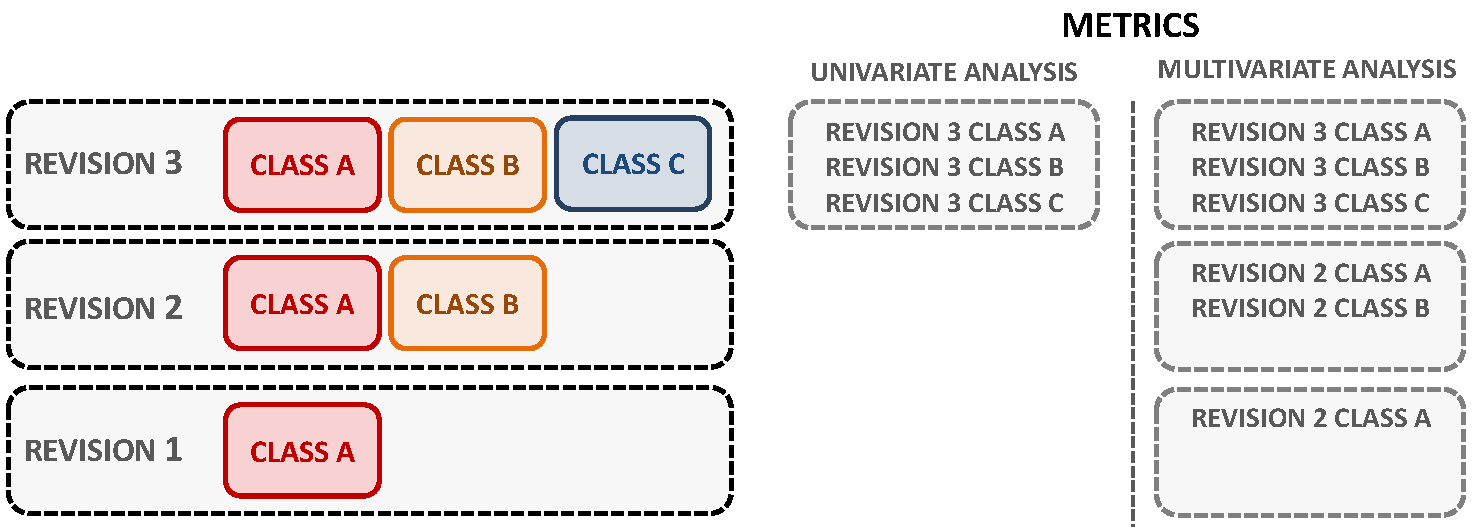
\includegraphics[width=1.0\textwidth]{AnalysisDataSets.pdf}
\caption{An illustration of the difference between data sets for each of the univariate and multivariate analysis.}
\label{fig:AnalysisDataSets}
\end{figure}

\section{Sample Analysis} %Section - 4.3 
Ahead of conducting a detailed analysis of the \textit{sample} or carrying out a regression analysis to answer the research questions, it is standard practice to conduct an initial exploratory data analysis. This is a typical approach in this type of research  \citep{grechanik2010empirical, cartwright2000empirical} as it enables for a dissection of the dataset allowing it to reveal its underlying structure without prior assumptions or biases. It is through that initial analysis that potential complexities or threats to validity can be identified mitigated \citep{tukey1977exploratory}. This section details that exploratory data analysis as applied to the \textit{sample} of 658 projects and presented against similar analysis in the \textit{population} of 22,594 projects. This analysis will show that the sample is broadly representative of the wider forge.

\subsection{Exploratory Data Analysis}
First, the extensions of files contained within the commits were mined and analysed with the results confirming a very heavy bias towards the Java file extension alongside other file extensions usually associated with Java web-based projects. This is as expected given the project sample selection criteria which exclusively selected 'Java' tagged projects. The results of this analysis are depicted in Table ~\ref{tab:GoogleCodeExtensions}. The table reveals a substantial proportion of XML files (typically used in Java projects  for configuration) and HTML and graphics files (mostly used in web-based projects).

\begin{table}
\centering 
\captionof{table}{File Extensions: top five cumulative occurrences.}
\begin{tabular}
 \centering 
 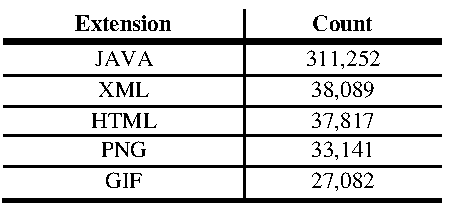
\includegraphics{GoogleCodeExtensions.pdf}
 \label{tab:GoogleCodeExtensions}
\end{tabular}
\end{table}

Next, the cumulative number of project committers was analysed. This is of relevance to this analysis as it is used as a measure of team size. Figure ~\ref{fig:CumulativeCommitterCount} shows that the sample follows a similar profile to the forge-wide analysis. Table ~\ref{tab:SampleTeamSizes} summarises the project team sizes in greater detail. The analysis reveals that more projects exist on lower committer counts; a fact that will have a bearing on the upper limit imposed on team size throughout the analysis in this chapter to help ensure a substantial population of data points for each team size that is included in this study.

\begin{figure}[htbp!] 
\centering    
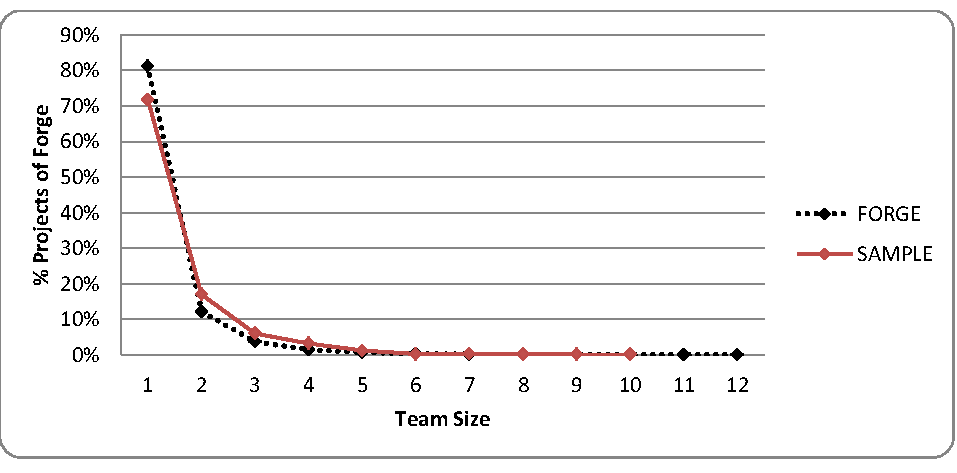
\includegraphics[width=1.0\textwidth]{CumulativeCommitterCount.pdf}
\caption{The number of projects with a team size of 1, 2, 3 through to 12.}
\label{fig:CumulativeCommitterCount}
\end{figure}

\begin{table}
\centering 
\captionof{table}{The number of projects within the sample of 658 projects, grouped by team size.}
\begin{tabular}
 \centering 
 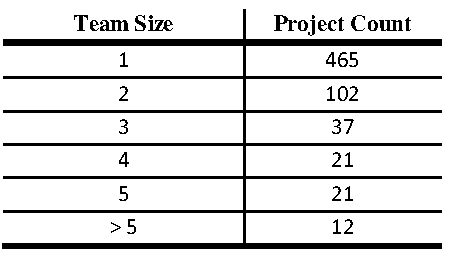
\includegraphics{SampleTeamSizes.pdf}
 \label{tab:SampleTeamSizes}
\end{tabular}
\end{table}

Committer behaviour was also analysed by investigating the cumulative number of commits grouped by committer and project, depicted in Figure ~\ref{fig:CommitCountBarChart}. It is notable that the broader forge shows a majority of committers only ever contributing a single commit when participating in a project. The sample deviates from this trend exhibiting a more even distribution across committer activity levels. This is attributable to the fact that the sample constituting only those projects tagged with the appropriate meta-data and, hence, are more likely to be active projects showing more sustained committer engagement. These trends will bear relevance to the multivariate team analysis later in this chapter where structural metrics are grouped by the number of revisions that files undergo.

\begin{figure}[htbp!] 
\centering    
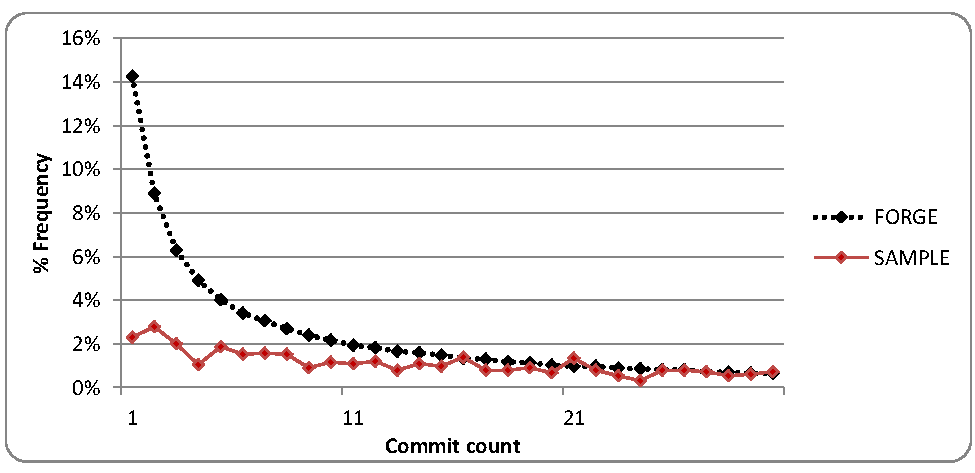
\includegraphics[width=1.0\textwidth]{CommitCount.pdf}
\caption[The number of commits that each committer makes within individual projects]{Sample analysis of the number of commits that each committer makes within individual projects. The chart shows  x-axis shows the number of commits that a committer contributes to a project and the y-axis shows the frequency of that level of project engagement.}
\label{fig:CommitCountBarChart}
\end{figure}

The final aspect of sample analysis concerns the nature of the individual commits that make up committer activity. An individual commit can have any number of affected files. A commit could be a single file or path modification or, on the other extreme, the check-in of large mature codebase. Figure ~\ref{fig:AffectedFiles} shows the general trend that smaller commits are more frequent than larger ones. Any file-level analysis of commit information will necessitate the joining the structural metrics of potentially multiple affected files with the commit-level data. This will become apparent through the course of the multivariate team analysis.

\begin{figure}[htbp!] 
\centering    
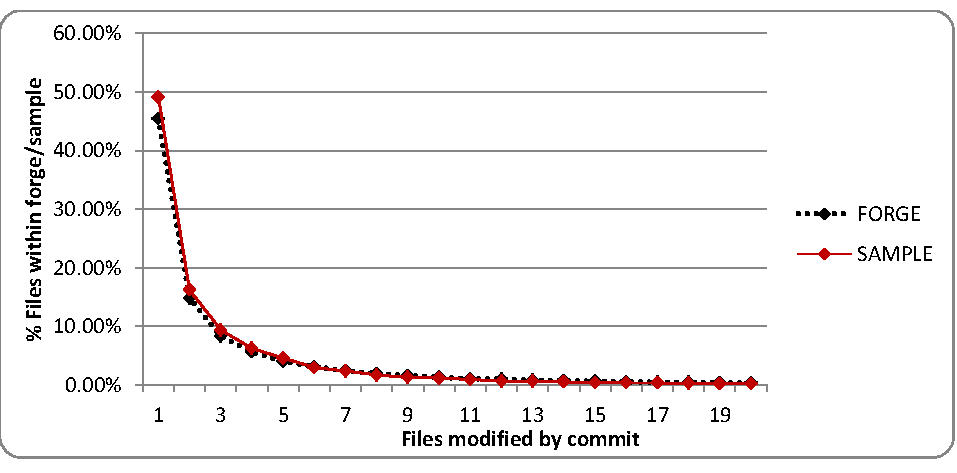
\includegraphics[width=1.0\textwidth]{AffectedFiles.pdf}
\caption{The frequency of commits grouped by the number of files affected.}
\label{fig:AffectedFiles}
\end{figure}

\subsection{Distributions and Correlations}
To conduct robust hypothesis testing and apply linear regression techniques, it is necessary to understand how the key parameters of the data set distribute relative to a normal distrubtion. An in-depth qualitative analysis of the distributions of CK metrics is not the focus of this work and the reader is referred to the work of Succi et al. \citep{succi2005empirical} and Basili et al. \citep{basili1996validation} for an analysis into the typical distribution of CK metrics for Java and C++ software respectively. For the purposes of this research the Kolmogorov-Smirnov test was used to compare the population of values of each CK metric against a normal distribution \citep{kolmogorov1933sulla, smirnov1948table}. This test makes no assumptions of the distribution of those data sets being compared and produces a p-value and a D-statistic as an output. Table ~\ref{tab:KSTest} shows zero p-values allowing the rejection of the null hypothesis of normality. The D-statistic indicates the ratio of the data sets that exists outside the normal distribution. This insight will influence the choice of statistical methods later in this thesis.

To analyse the relationship between the metrics within the sample, the Spearman correlation coefficients are analysed in Figure ~\ref{tab:MetricCorrelations}. The Spearman measure of correlation was chosen as it makes no assumptions of the normality of the distribution of the data being analysed \citep{spearman1904proof}. The correlation matrix shows positive correlations between CBO, LCOM, RFC and WMC. Weak correlations exist DIT, NOC and the remainder of the metrics. These observations are in-line with prior analysis by Succi et al. \citep{succi2005empirical}. Team size is found to be correlated to CBO and, to a lesser extent DIT, NOC and RFC. It is worth stressing that, for reasons explained in the next section, team size is measured at a project level while the metric values are at an individual class level. This initial result implies that greater team sizes cause metrics to trend counter to the objective as articulated by Rosenberg and others (detailed earlier in Chapter 2) - something which has been empirically associated with degraded external attributes. This adds further weight to the empirical evidence of prior research associating larger team sizes to lower productivity \citep{pendharkar2009relationship} and greater fault-proneness \citep{nagappan2008influence, caglayan2015merits}.

\begin{table}
\centering 
\captionof{table}{Results of Kolmogorov-Smirnov tests comparing the distribution of each metric against a 'reference' normal distribution.}
\begin{tabular}
 \centering 
 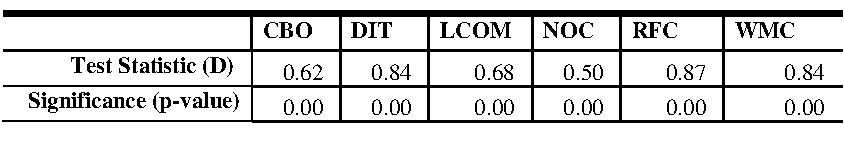
\includegraphics{KSTest.pdf}
 \label{tab:KSTest}
\end{tabular}
\end{table}

\begin{table}
\centering 
\captionof{table}{Spearman correlation matrix for Team Size and the CK metrics within the sample.}
\begin{tabular}
 \centering 
 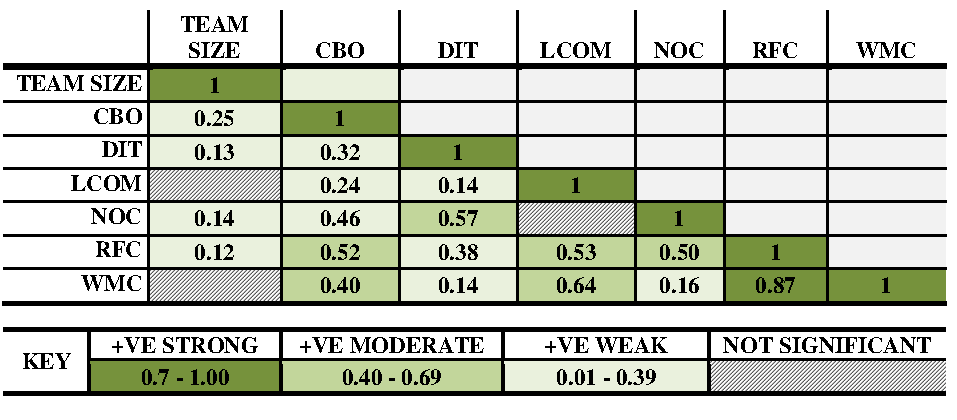
\includegraphics[width=1.0\textwidth]{MetricCorrelationsSpearman.pdf}
 \label{tab:MetricCorrelations}
\end{tabular}
\end{table}


\section{Univariate Team Size Analysis} %Section - 4.4
\subsection{Defining the Team Size}
For the purpose of this research, team size is defined as the cumulative total of all unique committers present in the revision history in the version control system of a given project. 

As alluded to in the previous section, while it is reasonable to suggest that such a definition would be an oversimplification as some committers could contribute to the codebase during widely varying time windows, it was posited that the majority do commit in overlapping time windows. This is borne out in analysis of the project sample that found that 83\% of committers to a project contribute in overlapping time windows to their fellow contributors, an example of which is shown in Figure ~\ref{fig:TeamSizeExample}. This fact, alluded to the reality that those committers who contribute outside the time window of their peers nevertheless leave an impact to the codebase which cannot be discounted, reinforces the argument in favour of a simple cumulative measure of team size.

Mockus et al. studied an Apache project and observed that the majority of development was attributable to a minority of 'core' developers \citep{mockus2000case} who commit frequently to the codebase. It could be suggested that the measure of team size proposed in this research does not distinguish between this frequent core committers and infrequent 'peripheral' committers. As Figure ~\ref{fig:CommitterCommitCount} illustrates, a significant amount of activity takes place by those committers who contribute with a low number of commits, hence infrequent committers cannot be excluded from any analysis without losing a key influencing factor on the codebase. Indeed Terceiro et al. studied the contributions of core and peripheral committers across 7 projects concluding that peripheral committers contribute a disproportionately high amount of structural complexity to the codebase further strengthening the argument that a measure of team size should include all committers \citep{terceiro2010empirical}. Figure ~\ref{fig:TeamSizeExample} highlights the simple and intuitive nature of a team size measure derived from the cumulative committer count as contrasted with a count of the number of committers with overlapping committer activity.

It is also reasonable to suggest that, given CK metrics are measured at an individual class level, so team size could also be measured at a class level (perhaps as the total number of committers to modify a class). This runs somewhat counter to the intention of making this research relevant to practitioners (particularly middle-management) which, the author argues, would relate much more to a measure of team size at a project level than at a class level.

\begin{figure}[htbp!] 
\centering    
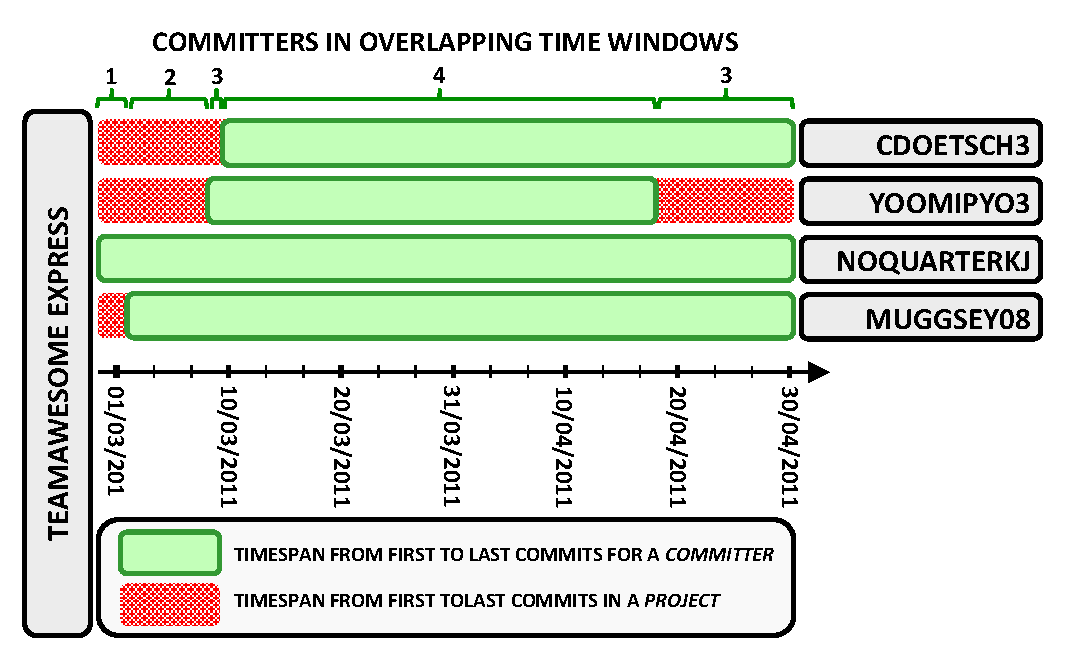
\includegraphics[width=1.0\textwidth]{TimeSizeExample.pdf}
\caption[The committer engagement timelines for project 'TeamAwesomeExpress'.]{The committer engagement timelines for project 'TeamAwesomeExpress'. The diagram depicts the count of the number of committers with overlapping timelines of activity.}
\label{fig:TeamSizeExample}
\end{figure}

\begin{figure}[htbp!] 
\centering    
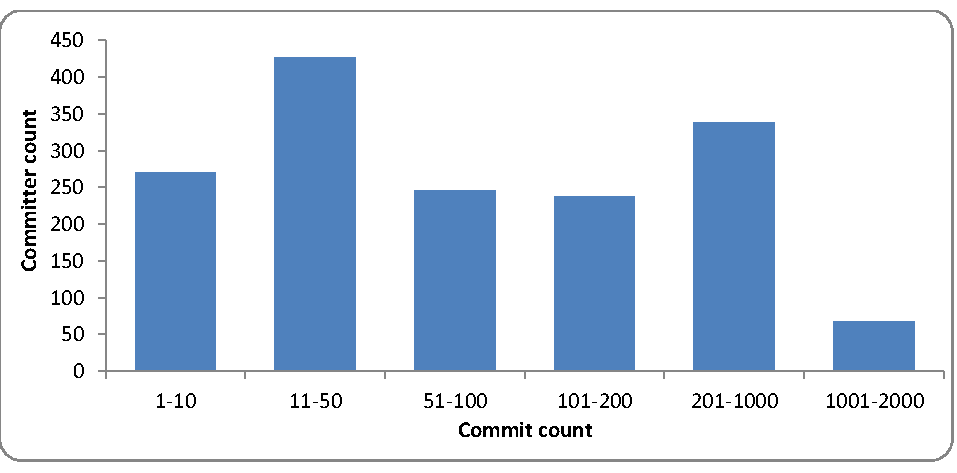
\includegraphics[width=1.0\textwidth]{CommitterCommitCount.pdf}
\caption{The number of commits that each committer makes within individual projects.}
\label{fig:CommitterCommitCount}
\end{figure}

\subsection{Analysis}
The analytical approach to the 'univariate' team size analysis uses, as its structural metric data set, the results of a static analysis of the projects codebases snapshotted at their final revisions. This is depicted in Figure ~\ref{fig:BasicAnalysisMetricMining} and illustrates the approach of overlooking the evolutionary path that a project took to reach its final (snapshotted) end state.

\begin{figure}[htbp!] 
\centering    
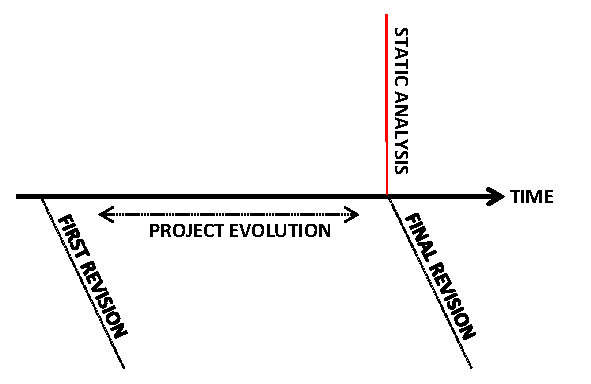
\includegraphics[width=0.7\textwidth]{BasicAnalysisMetricMining.pdf}
\caption{The evolution of project along the axis of time overlaid with a depiction of the point at which static analysis is conducted.}
\label{fig:BasicAnalysisMetricMining}
\end{figure}

Armed with these structural metrics, project metrics are then grouped or 'bucketed' according to the cumulative number of committers to the originating project. By way of example, should the total number of committers for a project number \textit{n}, then all the class-level structural metrics for that project would move into the \textit{n} committers bucket. This is illustrated in Figure ~\ref{fig:BasicBucketingStrategy}.
 
\begin{figure}[htbp!] 
\centering    
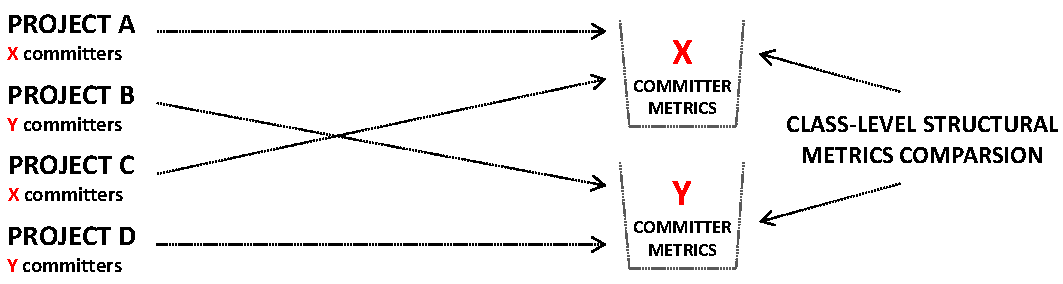
\includegraphics[width=1.0\textwidth]{BasicBucketingStrategy.pdf}
\caption{An illustration of our bucketing strategy categorizing the class-level structural metrics of a project according to the cumulative committer count of that project.}
\label{fig:BasicBucketingStrategy}
\end{figure}

As shown in the sample analysis in Figure ~\ref{fig:CumulativeCommitterCount} earlier, there is a dramatic drop in the proportion of projects that have a higher committer count compared with those projects with a lower committer count. In the sample this drop is particularly dramatic from 5 committers to 6 committers with counts of 12 and 3 projects respectively. For this reason, the statistical analysis excludes buckets for 6 or more committers. As will be discussed in Chapter 6, this can present an external threat to validity generalising some of the findings in this research to substantially larger team sizes. 

\begin{table}
\centering 
\caption{The bucketed metric comparison strategy.}
\begin{tabular}
 \centering 
 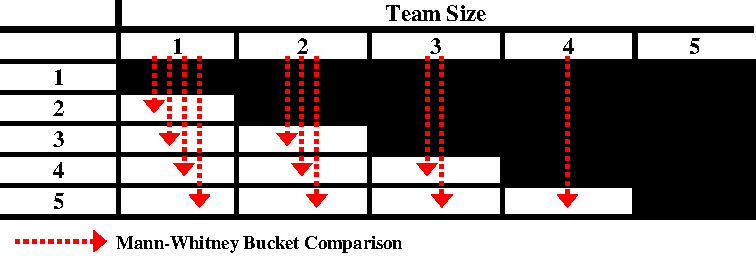
\includegraphics[width=1.0\textwidth]{MetricsComparisionStrategyTabular.pdf}
 \label{tab:MetricsComparisionStrategyTabular}
\end{tabular}
\end{table}

Table ~\ref{tab:MetricsComparisionStrategyTabular} illustrates the approach of comparing each bucket to every other. When comparing metrics populations bucketed by committer count, the Mann-Whitney test is ideally suited as all metrics populations are independent and consist of continuous non-normal data \citep{mann1947test}. Unlike the t-test, the Mann-Whitney test is a null hypothesis test that makes no assumptions of the distribution of the data. Null hypothesis H0,1 anticipates no significant difference between bucket populations of varying committer count and is rejected where the p-value is less than a certain threshold denoted by $\alpha$. With a target confidence level of 95\% this would imply a p-value cut-off ($\alpha$) at 0.05. However, a number of hypothesis tests are conducted, increasing the likelihood of observing at least one significant result at our chosen value of $\alpha$. It is therefore necessary to apply the 'Bonferroni correction' which sets the significance cut-off at the product of $\alpha$ and \textit{n} where \textit{n} represents the number of tests \citep{bonferroni1936teoria}. In this analysis there are 10 hypothesis tests for each metric giving a corrected $\alpha$ value of 0.005. Where the null hypothesis is rejected, the mean value of the bucketed metric populations are compared to determine in which direction the metric value is trending. Table ~\ref{tab:BasicResultsAverages} shows the mean and median metric values and observation counts by bucket.

Table ~\ref{tab:BasicResultsSignificance} summarises the results of this analysis, based on which, two immediate observations can be made.

\begin{itemize}
\item  \textbf{Rejecting null hypothesis H0,1:} The null hypothesis can be rejected in the case of all metrics with the exception of NOC as p-values are lower than the  $\alpha$ for most of the remaining metrics comparison tests. NOC excepted, 44 out of 50 comparisons show p-values under the $\alpha$ threshold. 
\item  \textbf{Metrics not overwhelmingly trending in a one direction:} Based on the analysis of simple means, there is a roughly even split between metric values increasing in value by committer count and those decreasing in value. Looking at the trends in more detail, DIT and RFC bucket comparisons show a dominant trend of decreasing metric values with increasing committer count. However, DIT shows the opposing trend where 1 committer bucket is compared to 2, 3, and 4 committer buckets. Similarly, the LCOM bucket comparisons show a dominant trend of increasing metric values with increasing committer count.
\end{itemize}

While some trends do emerge from this analysis, it is important from the perspective of the validity of this research to ascertain whether there are any potentially confounding factors that may be impacting these results. That is the subject of the next section.

\begin{table}
\centering 
\captionof{table}{Tabular summary showing the results of each bucket comparison within the sample analysis.}
\begin{tabular}
 \centering 
 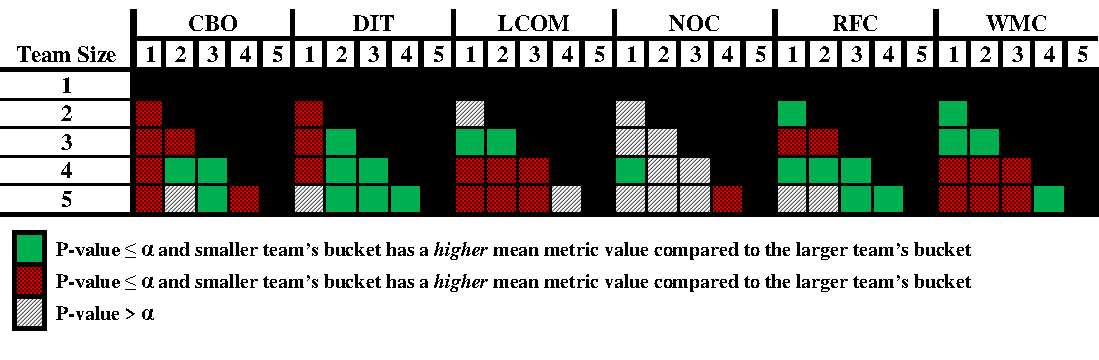
\includegraphics[width=1.0\textwidth]{BasicResultsSignificance.pdf}
 \label{tab:BasicResultsSignificance}
\end{tabular}
\end{table}

\begin{table}
\centering 
\captionof{table}{Metric mean and median values for each metric bucket within the sample analysis.}
\begin{tabular}
 \centering 
 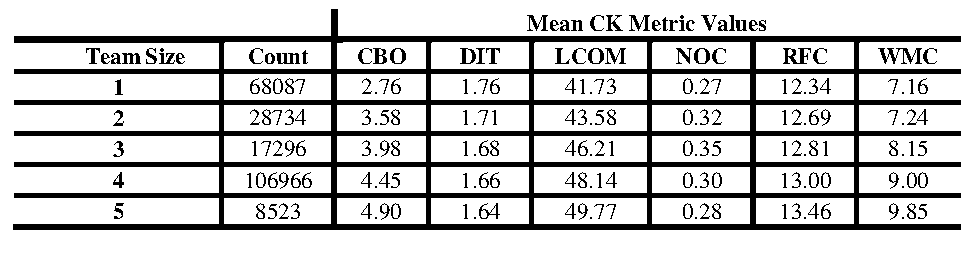
\includegraphics[width=1.0\textwidth]{BasicResultsAverages.pdf}
 \label{tab:BasicResultsAverages}
\end{tabular}
\end{table}

\subsection{Confounding Factors}
Confounding factors are those that influence both the dependent and independent variables within a model causing an association to be made which may not be genuine. In prior research modelling the impact of structural metrics on the externally observable attributes of software, class size was found to be one such factor. Emam et al. found that class size had a confounding impact on fault-proneness \citep{el2001prediction}. They suggested that earlier models which had established the predictive power of CK metrics over fault-proneness were largely (but not entirely) driven by class size and therefore not controlling for this confounding variable was a significant threat to validity. Their work was very recently corroborated by Gil and Lalouche \citep{gil2017correlation} who argued that this threat to validity also extends to other OO metrics. In a similar vein, Zhou and Leung found that class-size was a confounding variable to CK metrics models where change-proneness was the dependent variable \citep{zhou2006empirical}.

This research differs from the prior literature in that the CK metrics are essentially the dependent variables rather than the independent variables. For the purposes of the validity of this analysis, it is necessary to establish those factors that could potentially confound models that use CK metrics as the dependent variables.

\newline
\textbf{4.4.3.1 Class Size}
\newline
The typical measure of class size is  Lines of Code (or LOC). This is a simple measure of the number of lines within a class to the exclusion of comment lines \citep{nguyen2007sloc}. An analysis of the Spearman correlation p-values show no correlation between class-level LoC, team size and CK metrics. This is not surprising in an object-oriented language where one could reasonably hypothesise that a larger team is likely to work on a codebase which has more class files rather than larger class files per se. Similarly, LOC shows very weak negative correlations to the DIT and NOC metrics with almost no correlation to the rest of the metrics. On this basis it is accurate to say that class size has no relationship to either the dependent or independent variables in the model that was established in the previous section and therefore cannot be considered a confounding factor that should be controlled. Figure ~\ref{fig:AllMetricsAgainstLOC}  depicts how CK metrics trend against project size showing the mean metric values across individual projects against their aggregate Lines of Code (LOC) count. These charts show that at a project level there is no obvious relationship between code volume and metric values.

\begin{figure}[htbp!] 
\centering    
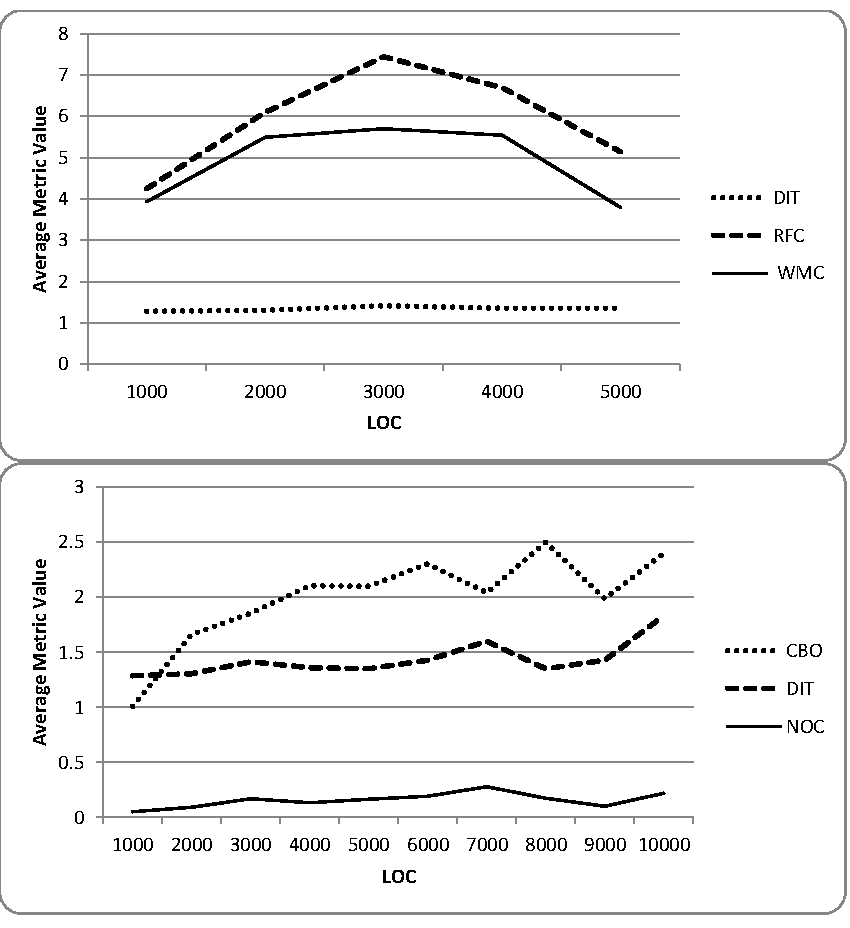
\includegraphics[width=1.0\textwidth]{AllMetricsAgainstLOC.pdf}
\caption{Sample analysis of the mean project-level structural metric values plotted against the cumulative Lines of Code for that project.}
\label{fig:AllMetricsAgainstLOC}
\end{figure}

\newline
\textbf{4.4.3.2 Revision Counts}
\newline
When using version control systems, it is usual to build functionality iteratively through repeated modification of source files. This represents the development iterations driving the evolution of the codebase. It has been proven that, as software projects evolve, iterations of a codebase tend to exhibit both growing size and complexity \citep{prather1984axiomatic}. Each time a file (or group of files) is edited and re-committed this is considered a single revision. Revisions are tagged with commit comments which often refer explicitly to additional functionality that relates to the commit. An example of this can be seen in Figure ~\ref{fig:PreciseRevisionLogs} which is an excerpt from the revision logs from a project called 'Precise', a requirements management tool, which will be studied in more detail in a later chapter.

\begin{figure}[htbp!] 
\centering    
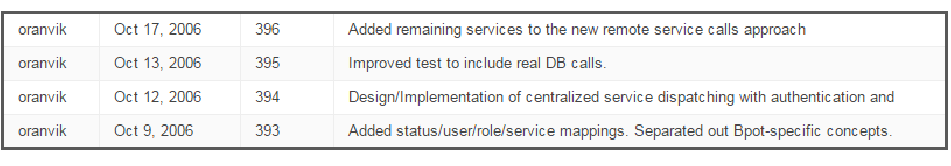
\includegraphics[width=1.0\textwidth]{PreciseRevisionLogs.pdf}
\caption{An excerpt of the revision log from the 'precise' project showing commentary explaining the addition of functional complexity with each revision.}
\label{fig:PreciseRevisionLogs}
\end{figure}

To date in this thesis, references to complexity have, in fact, alluded to structural complexity. This was defined earlier as the measure of the degree of interactions between components in a software system. This is in contrast to functional complexity which has no single definition but generally refers to the degree of sophistication in the logic encoded within a software system. Revision counts are an important factor to study as, this research argues, it represents a proxy to functional complexity (albeit a flawed one). While measuring structural complexity is a fairly straightforward task captured by RFC and WMC metrics (to make no mention of Halstead or McCabe's complexity metrics which are specifically designed for this purpose) capturing functional complexity is notoriously more difficult. Several measures have been proposed, generally with a tendency to conflate functional and structural complexity through attempts to track the nature of control structures within the source code or interactions between components. It is understandable that code inspection would be the default approach to measuring functional complexity as, where requirements are documented, they are often fragmented and therefore difficult interpret in an automated fashion. 

Revision counts cannot be considered a perfect proxy to functional complexity as revisions will not exclusively be associated with the addition of new logic. Refactoring activities and bug fixes both necessitate revisions which would not add to the functional complexity. The efficacy of revision counts as a proxy to functional complexity is beyond the scope of this work but, nonetheless, revision counts are an important factor worthy of further study for its potential confounding effect.

Table ~\ref{tab:RevisionCorrelations} shows the Spearman correlation coefficients for the relationship of revisions to team size and also CK metrics. It is notable that revisions do have a marked positive correlation to team size (0.47) as well as to the CK metrics; particularly CBO and RFC (0.29, 0.21 respectively). While these correlations are weak (under the arbitrary threshold of 0.40) they are nonetheless significant and imply a linear relationship between revisions and both the independent and dependent factors in our earlier model; namely team size and CK metrics respectively.

\begin{table}
\centering 
\captionof{table}{Sample analysis of the Spearman correlation coefficients for revisions against team size and each CK metric.}
\begin{tabular}
 \centering 
 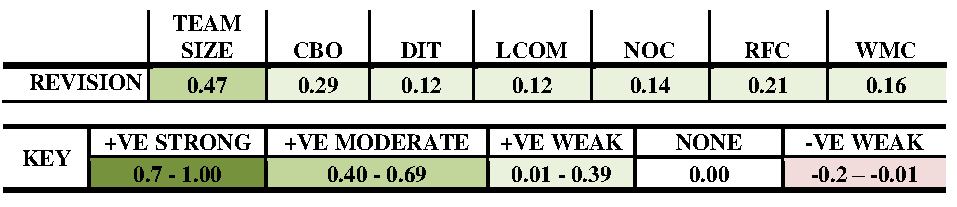
\includegraphics[width=1.0\textwidth]{RevisionCorrelationsSpearman.pdf}
 \label{tab:RevisionCorrelations}
\end{tabular}
\end{table}

This relationship between revisions and team size is confirmed at a project level with Figure ~\ref{fig:RevisionsCommitters} showing that the cumulative number of committers to a project trending positively against the number of revisions that the project has undergone. Furthermore, Figure ~\ref{fig:MetricsRevisions} demonstrates a clear positive correlation between class revision counts and all CK metrics with the exception of DIT and NOC. These metrics capture a very specific facet of structural complexity - inheritance complexity - which the results imply is not correlated with functional complexity. These results are consistent with the work of Johari et al. \citep{johari2012validation} who studied the relationship between CK metrics and revision counts on an open-source project. 

\begin{figure}[htbp!] 
\centering    
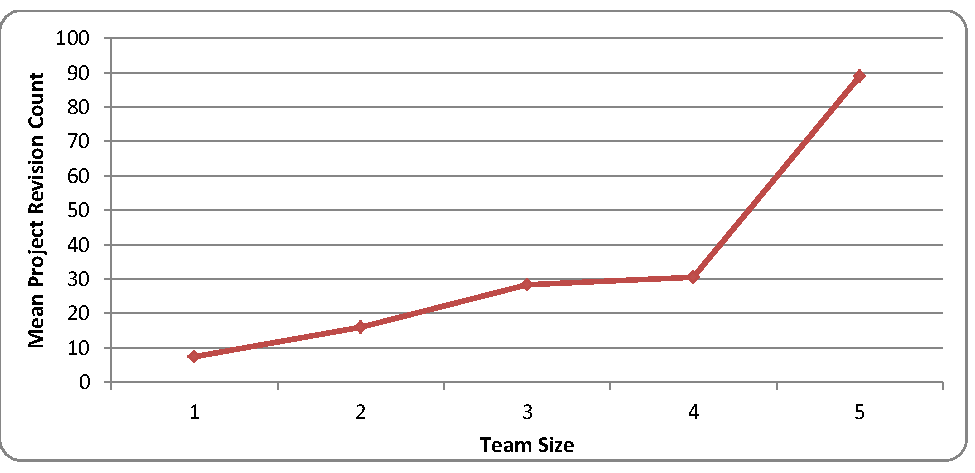
\includegraphics[width=1.0\textwidth]{RevisionsCommitters.pdf}
\caption{Analysis of the sample projects showing a clear upwards trend of the project revision count against committer count.}
\label{fig:RevisionsCommitters}
\end{figure}

\begin{figure}[htbp!] 
\centering    
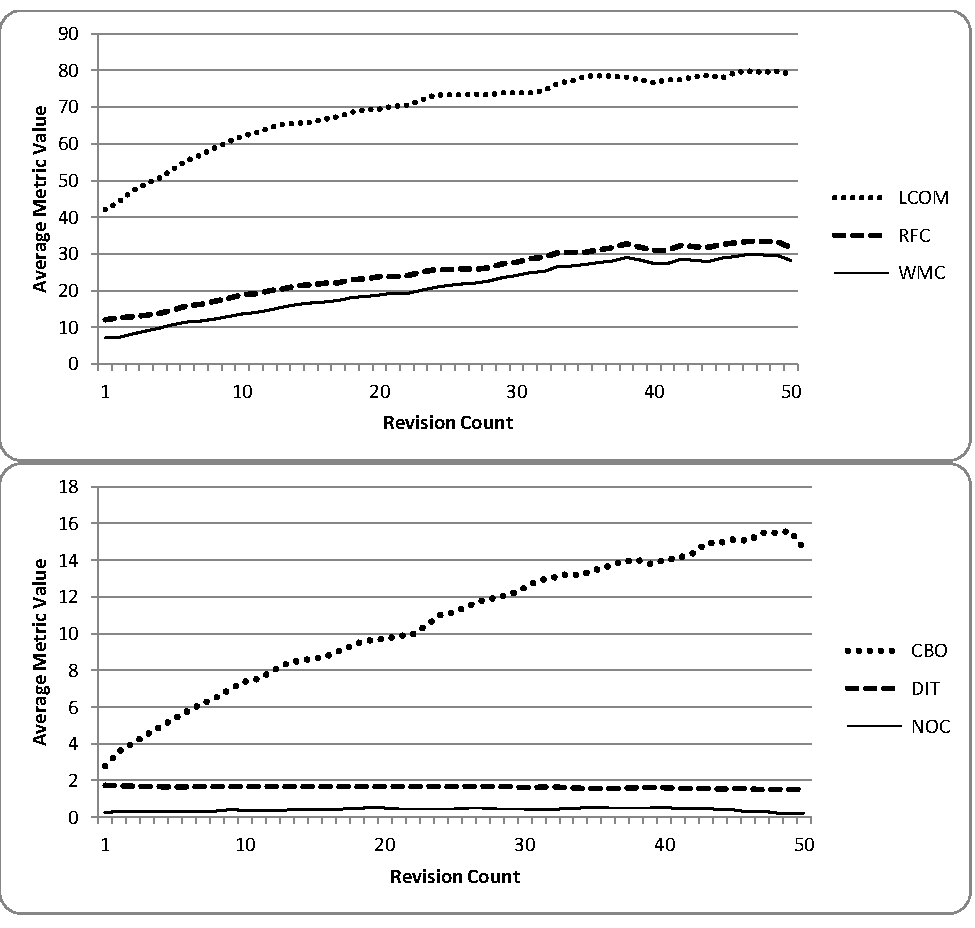
\includegraphics[width=1.0\textwidth]{MetricsRevisions.pdf}
\caption{Mean metric values at a class level plotted against the last revision count for all files within the sample.}
\label{fig:MetricsRevisions}
\end{figure}

\section{Multivariate Team Size Analysis} %Section - 4.6

\subsection{Data Analysis Approach}
Having established revision counts as a confounding factor, in order to accurately study the impact of team size and produce reliable comparisons between metric populations of varying committer count it is necessary to control for revision counts. Continuing with the same sample as previously described, the data set takes the form of a class-level and revision-level CK metrics along with date and committer associated with each file revision as previously illustrated in ~\ref{fig:PreciseRevisionLogs}. This allows the determination of the number of unique committers to an individual project which is, as defined earlier, the project development team size. The approach of conducting static data analysis at each revision of the projects in our sample is illustrated in Figure ~\ref{fig:AdvancedAnalysisMetricMining}. This figure depicts the evolution of a project revised through its timeline of development with each revision the subject of static code analysis. 

\begin{figure}[htbp!] 
\centering    
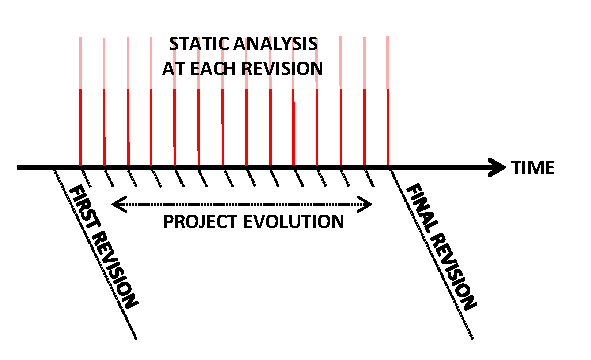
\includegraphics[width=0.7\textwidth]{AdvancedAnalysisMetricMining.pdf}
\caption{Static analysis is conducted at each revision of the project evolution.}
\label{fig:AdvancedAnalysisMetricMining}
\end{figure}

Given this enriched data set, metrics can be grouped together by project team size - irrespective of the individual project from which they came - and considered distinct populations. For example, if project X and project Y each had the same number of unique committers, all metrics belonging to each file within both projects would reside in a single bucket. Using this bucketing approach, a set of distinct metrics populations can be compared using statistical techniques. From the meta-data associated with each file, the number of revisions any one file has undergone can be ascertained. This data will feed into the bucketing process where the population of metrics within a particular bucket only contains those metrics belonging to projects with a particular team size and only from files that have been modified a particular number of times. This approach, illustrated in Figure ~\ref{fig:AdvancedBucketingStrategy}, will give confidence that, when comparing our bucketed metric populations, any statistically significant differences are attributable to team size without the confounding impact of revisions.

\begin{figure}[htbp!] 
\centering    
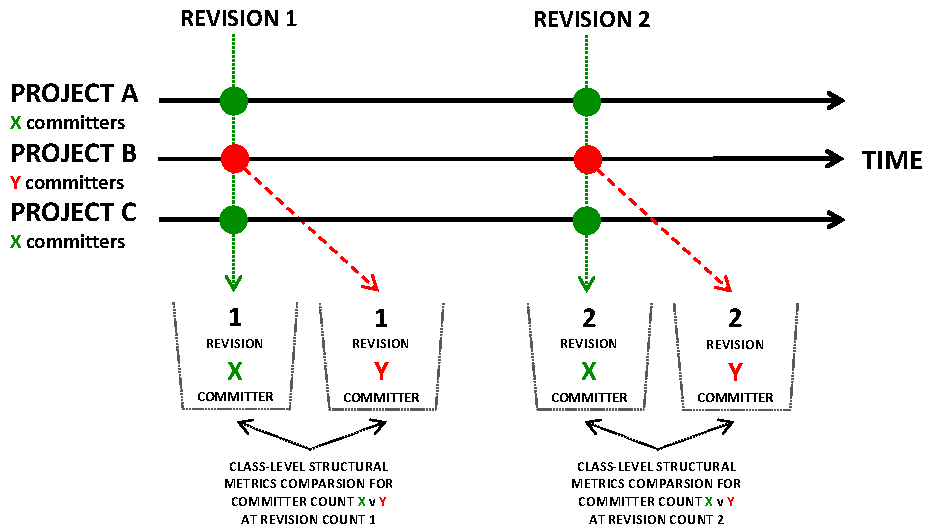
\includegraphics[width=1.0\textwidth]{AdvancedBucketingStrategy.pdf}
\caption{An illustration of the bucketing approach used to categorise metrics for comparison.}
\label{fig:AdvancedBucketingStrategy}
\end{figure}
	
Consistent with the univariate team analysis in the previous section, as the dimensions in the data are not normally distributed, the Mann-Whitney test is again used to compare bucketed populations of metrics. Once again null hypothesis H0,1 is the subject of this analysis. H0,1 is rejected where the bucketed populations are found be independent where the p-values indicate a 95\% confidence level. As 50 hypothesis tests are executed for each metric, once again the Bonferroni correction need apply. This sets the p-value threshold of $\alpha$ at 0.001.

It is logical that there would be a greater number of metric results pertaining to the lower revision counts as, by necessity, for a file to be revised \texit{x} times, it would have \texit{x}-1 prior revisions (where \texit{x}>1). However, it is perfectly normal for a file to only have very few total revisions. This is an important consideration as those buckets with metric populations of higher revisions and committer counts have diminishing populations. Figure ~\ref{fig:MetricsPopulationRevisions} and table ~\ref{tab:BucketPopulations} show this effect. For this reason, and to ensure suitable metric populations in each bucket, in this analysis only buckets belonging to team up to 5 committers with a maximum of 6 revisions are considered. A substantial drop in bucket population is notable beyond these thresholds.

\begin{table}
\centering 
\captionof{table}{Bucket population sizes where each file within the sample is inspected at its final revision.}
\begin{tabular}
 \centering 
 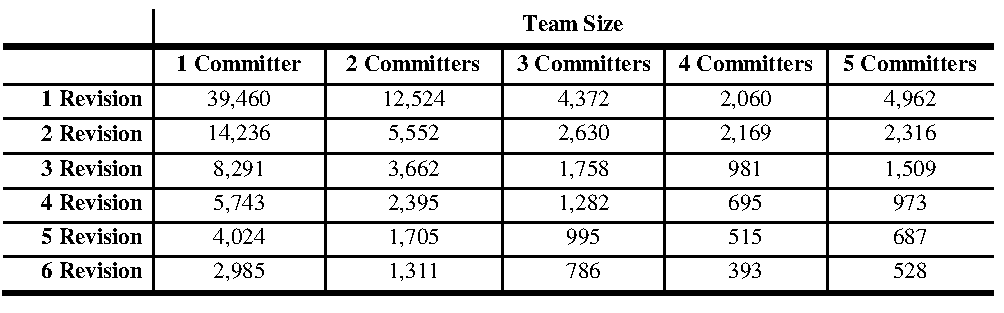
\includegraphics[width=1.0\textwidth]{BucketPopulations.pdf}
 \label{tab:BucketPopulations}
\end{tabular}
\end{table}

\begin{figure}[htbp!] 
\centering    
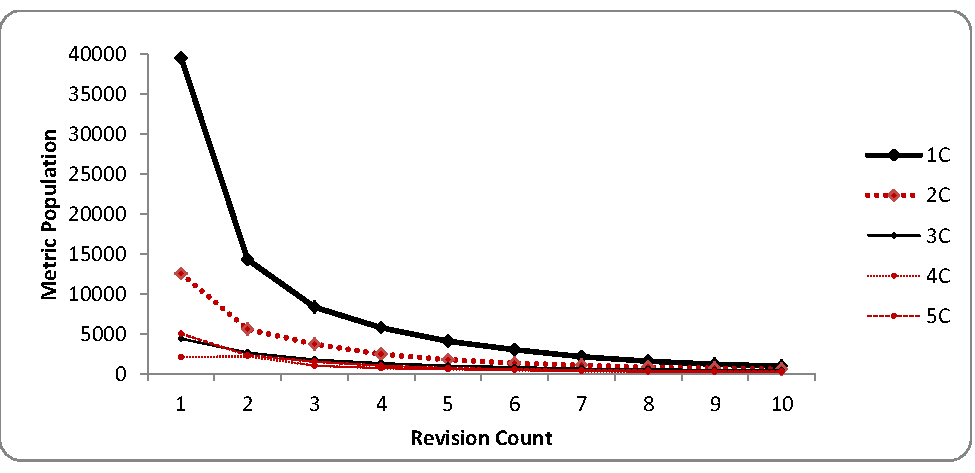
\includegraphics[width=1.0\textwidth]{MetricsPopulationRevisions.pdf}
\caption{Analysis of mean metric values against revision count where each file within the sample is inspected at its final revision.}
\label{fig:MetricsPopulationRevisions}
\end{figure}

\subsection{Comparing Bucket Populations}
Table ~\ref{tab:ComplexResultsBucketComparisions} shows the results from the statistical tests run across each team-size comparison, similar to the previously discussed Table \ref{tab:BasicResultsSignificance} but also grouped by revision. By way of explanation, the first set of rows are bucket comparisons for the CBO metric. The revision columns relate to the number of times that the classes (from which the metrics were extracted to make the bucket metric populations) have been revised. The committer count columns and rows refer to the number of unique committers to the project from which the class originates. For completeness, those tests that do not meet the Bonferroni corrected $\alpha$ cut-off but do show significance at the 95\% confidence level are depicted accordingly. 

Where the bucket populations are found to be significantly independent the bucket population metric means are compared. Based on this, a determination is made as to whether increasing committer count will result in a rise or a fall in the metric value.

From these results a number of notable observations can be made. 

\begin{itemize}
\item  \textbf{Rejecting null hypothesis H0,1:} After controlling for revisions it is still possible to reject null hypothesis H0,1 for all metrics but NOC and RFC. NOC showed no impact from team size before or after controlling for revision counts. However, RFC did earlier show a negative association with team size but this analysis has shown that this was due to the confounding impact of revision counts.  It is evident that a large number of buckets that show statistical significance across CBO, LCOM, WMC and, to a lesser extent, DIT.

\item  \textbf{DIT and LCOM show a positive relationship with team size at higher revisions:} The results for DIT and LCOM show a dominant trend of increased committer count resulting in increased metric values. In the case of DIT this trend is stronger at higher revisions of 4 and above. However, DIT does the opposing trend where 1 committer bucket is compared to 2, 3, and 4 committer buckets. Similarly, the LCOM bucket comparisons show a dominant trend of increasing metric values with increasing team size.

\item  \textbf{WMC shows a negative association with team size:} WMC shows a  trend with a decrease in metric value accompanying an increase in team size. 
\end{itemize}

\begin{table}
\centering 
\caption{Tabular summary showing the results of each bucket comparison within the sample.}
\begin{tabular}
 \centering 
 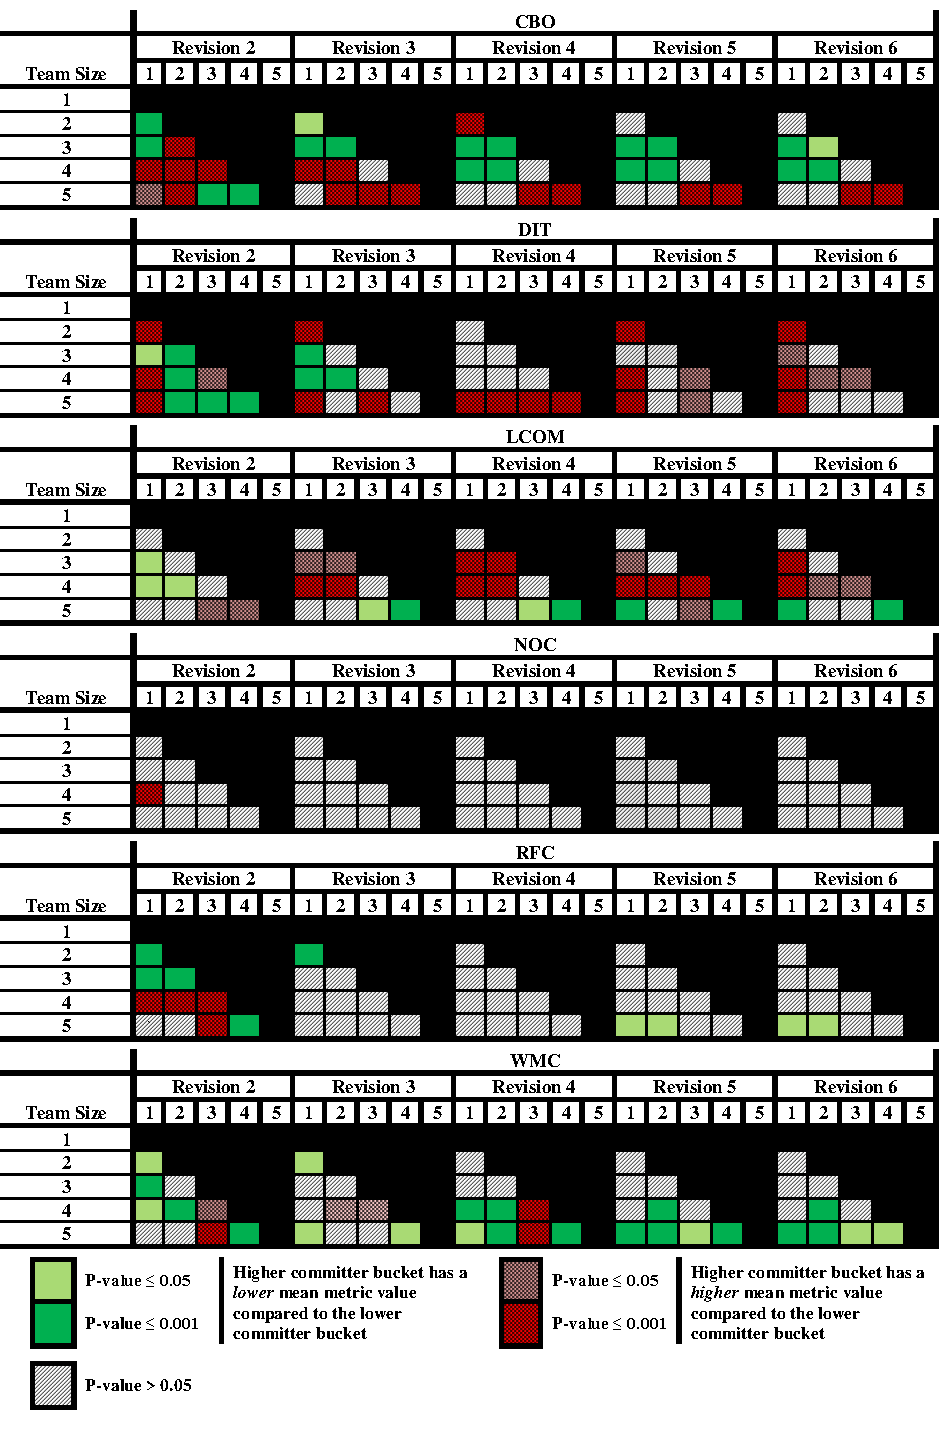
\includegraphics[width=1.0\textwidth]{ComplexResultsBucketComparisions.pdf}
 \label{tab:ComplexResultsBucketComparisions}
\end{tabular}
\end{table}

\subsection{Simple Linear Models}
While the previous analysis focussed on holding revision counts constant, it is appropriate to model revision counts and committer counts as two independent variables with the CK metric values being their dependent variables, using simple linear regression to analyse their impact. Table ~\ref{tab:TeamSizeBasicLinearRegression} shows the output of this linear regression using the Ordinary Least Squares (OLS) regression method. One of the considerations when using this method for multivariate regression is that collinearity between the independent variables can lead to misleading coefficient estimates. The Variance Inflation Factor measures the increase of the variance of the parameter estimates if an additional variable is added to the linear regression. This helps ascertain the impact of collinearity of parameters on the validity of an OLS regression. At 1.65, this measure is significantly less than the 'rule of thumb' threshold of 5 \citep{menard2002applied}, hence the collinearity between revisions and team size is not a concern.

The linear models capture the linear relationship between team size, class revision count (as independent variables) and CK metrics (as dependent variables) expressed as the following equation where team size and revision count are multiplied by their respective coefficients $\beta$, $\gamma$ is the intercept, and $\epsilon$ is the standard error:

\[\large Metric \: Value = \beta_{TS}\, TS +  \beta_{R}\, rev +  \gamma + \epsilon \]

\begin{table}
\centering 
\captionof{table}{The results of an Ordinary Least Squares regression using the sample dataset with committer and revision counts as independent variables.}
\begin{tabular}
 \centering 
 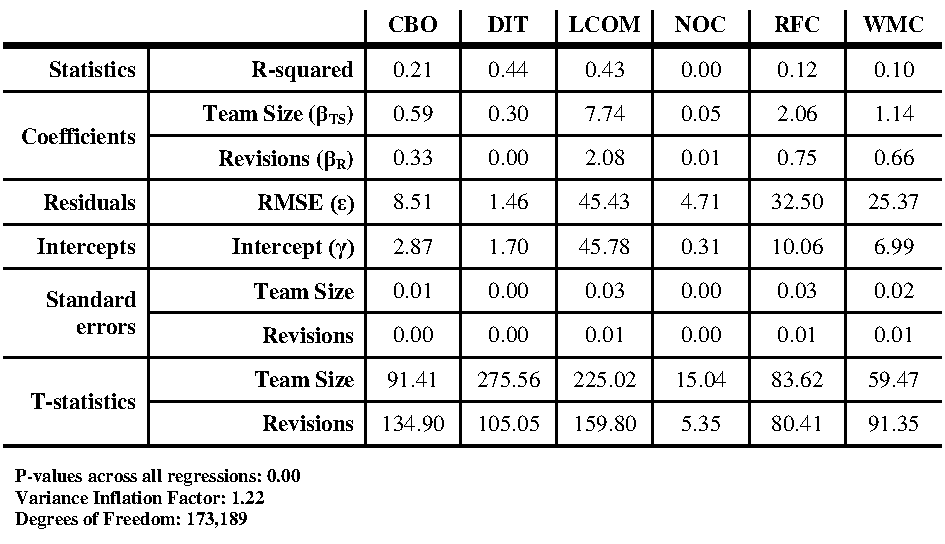
\includegraphics[width=1.0\textwidth]{BasicLinearRegression.pdf}
 \label{tab:TeamSizeBasicLinearRegression}
\end{tabular}
\end{table}

\textit{R-squared} is a statistical measure, ranging from '0' to '1', of how close the observed data points are to the fitted regression line. A value of '1' would imply that the independent variables linearly explain all variance of the respective CK metric.

The \textit{coefficients} are the estimated slope (that is to say the slope based on a sample of the population) of the component of the independent variable that is uncorrelated with the other independent variable. Coefficients cannot be directly compared across independent variables on the same model as they exist on different scales. For instance, if team size had the same impact on a metric value as revisions, it would still be expected that the coefficients of revisions would be lower given that they possess a higher range. Similarly it is not possible to directly compare coefficients of a specific independent variable across multiple CK metrics as here the dependent variables are on differing scales.

The \textit{residuals} are a measure of the distance between the actual observations and the model prediction. Table ~\ref{tab:TeamSizeBasicLinearRegression} shows the Root Mean Squared Error (RMSE) which is a measure of residuals in units of the respective CK metric. Residuals are difficult to interpret in isolation but will become useful when comparing the accuracy of these models against the mixed linear models in the next section.

The \textit{intercepts} are the values at which the fitted regression lines cross the y-axis. It is worth noting that the intercept point where team size and revisions are at '0' is purely a theoretical construct. It is useful, however, as it does indicate the degree to which the regression line is shifted upwards and will bear some relevance in Section 4.7 where intercepts of individual projects are compared.

\textit{Standard errors} indicate the degree to which the coefficient estimates may vary from the sample to the full population. This is a function of the \textit{R-squared} and the variance in the sample. \textit{T-statistics} are the ratio of the coefficient estimate and the standard error.  \textit{Degrees of freedom} are the number of independent observations available to establish a regression model.

The simple linear models detailed in Table ~\ref{tab:TeamSizeBasicLinearRegression} show a number of key results outlined as follows.

\begin{itemize}
\item  \textbf{Further rejection of null hypothesis H0,1:} In producing coefficients for team size and revisions, the linear modelling process first runs a hypothesis test to prove the rejection of the null hypothesis of coefficients of zero (i.e. the hypothesis that the independent variables have no effect on the dependent variables). This test returns highly significant p-values (approximated to 0.00) across all CK metrics.

\item  \textbf{Team size and revisions explain a substantial degree of variance, particular for DIT and LCOM:} It is notable that revisions and team size explain a substantial proportion of the variance in DIT and LCOM - 44\% and 43\% respectively - as represented by the R-squared values across the respective regression models. This is consistent with the results of the previous section that found that DIT and LCOM trended quite clearly positively with team size (controlling for revisions). NOC shows a R-squared value approximated to '0' which confirms the results of the spearman coefficient matrix that was presented earlier in Table ~\ref{tab:MetricCorrelationsSpearman} where no linear correlation was observed between NOC and the independent variables.

\item  \textbf{Inheritance complexity not impacted by revisions:} Coefficients close to zero for revisions across both DIT and NOC indicate that these metrics, both of which capture inheritance complexity, are not affected by revisions.

\item  \textbf{Team size trends positively with all CK metrics but NOC:} The positive estimated coefficients for team size ($\beta_{TS}$) across all regressions with the exception of NOC indicate that team size has a positive association with all but one of the CK metrics.

\item  \textbf{Low standard errors:} The standard errors indicate the probability that the sample mean and the population mean differ and therefore impact the estimated coefficients. The standard errors across the regression models do not rise above 0.03 indicating that, within a 97\% confidence level, the coefficients would prove accurate if calculated across the full population - i.e. all projects in the Forge.

\end{itemize}

\subsection{Linear Mixed Models}
While the application of the Ordinary Least Squares regression enabled the creation of some initial models, these models attempt to fit a single regression line per metric across the entire sample, disregarding the project-by-project variation. This is at odds with prior research which tends to produce a distinct population of observations for each project and study them individually using regression techniques (for the full survey refer to Tables ~\ref{tab:FaultModels} and ~\ref{tab:MaintainabilitySubatrributes}). This is somewhat intuitive as the idiosyncratic aspect of a project, driven by the nature and complexity of the functional behaviour as well as the individual programming traits of the individuals composing the team, has the potential to have a material impact on its structural metrics.

As this analysis is applied on a representative sample of an entire forge, it leads to a substantially larger data set than the 1-5 small/medium sized projects that is typical in the prior literature. As a result it is not feasible nor desirable to treat each project as an isolated data set as it would lead to a reduction in the degrees of freedom available to establish each individual linear model, consequently impacting the 'goodness of fit'.

Linear Mixed Models (LMMs) allow for a more nuanced linear regression by distinguishing between 'fixed effects' that apply to all groups and 'random effects' that apply individually to subgroups within data sets. Specifically, this approach can generate a single coefficient estimate but can allow for project-specific intercepts. This approach is useful in recognising and modelling the idiosyncratic 'project specific' impact to the metrics while using the full available data set to establish the coefficient estimates. 

This is the first application of LMMs to the study of software structural metrics but there is a substantial corpus of research that uses this technique in other fields. LMMs have gained recognition in the field of genomics for allowing 'relatedness' - modelled as the random effects - to factor in genetic association tests \citep{zhou2012genome}. Ecologists have recently started to apply this technique to modelling random effects of space, time and individuals in the study of species diversity and extinction risk \citep{bolker2009generalized}.

Linear mixed models can be expressed in a similar way to the previously specified OLS regressions in the previous section where $\gamma_p$ is now the \textit{project-specific} intercept:

\[\large Metric \: Value = \beta_{TS}\, TS +  \beta_{R}\, rev +  \gamma_p + \epsilon \]

Table ~\ref{tab:TeamSizeRandomInterceptsLinearRegression} summarises the results of a mixed model linear regression using project as the grouping variable. The coefficients and residuals are detailed as previously in the OLS regression results of Table ~\ref{tab:TeamSizeBasicLinearRegression}. The \textit{sample variance} shows the the degree to which observations are spread from the mean across the sample. The \textit{group variance} shows the same measure across individual groups and averaged across the full set of groups. This highlights the degree to which observations within a group share similar values when compared to ungrouped observations across the sample.

The following observations can be drawn from Table ~\ref{tab:TeamSizeRandomInterceptsLinearRegression}.

\begin{itemize}

\item  \textbf{Sample variance is substantially higher than group variance:} With the exception of the DIT regression, the groups exhibit lower variance than overall sample. This confirms that the  project-specific idiosyncratic characteristics have a significant bearing on metric values.

\item  \textbf{Lower Residuals:} The results from the LMMs exhibit substantially lower residuals across all metric regressions when compared to the OLS results in Table ~\ref{tab:TeamSizeBasicLinearRegression}. A reduction is expected as the intercepts are defined on a per project basis explicitly to reduce residuals.

\item  \textbf{Higher coefficient estimates:} The higher coefficient estimates in the LMMs indicate that team size and revisions have a greater impact on metric values than otherwise apparent in the OLS regression. While all projects share the same coefficient estimate, the revised values are attributable to the greater flexibility afforded by LMMs in fitting a regression line without forcing all projects through a single intercept.
\end{itemize}

\begin{table}
\centering 
\captionof{table}{The results of an mixed model linear regression against the sample dataset with committer and revision counts as independent variables and the project as the grouping variable.}
\begin{tabular}
 \centering 
 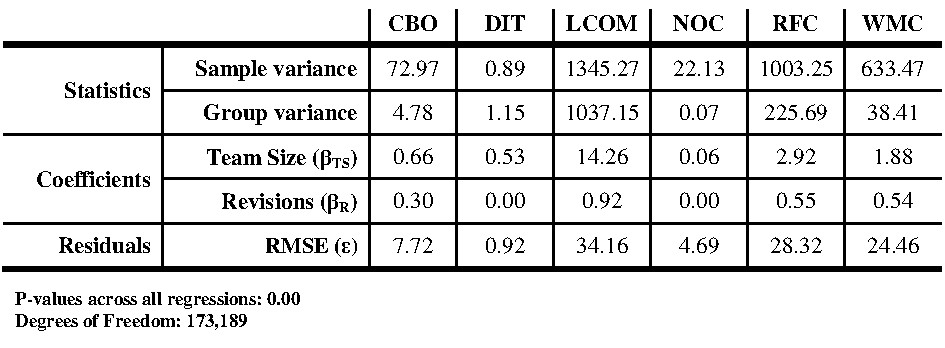
\includegraphics[width=1.0\textwidth]{RandomInterceptsLinearRegression.pdf}
 \label{tab:TeamSizeRandomInterceptsLinearRegression}
\end{tabular}
\end{table}

\section{Results at a Project Level} %Section - 4.9
\subsection{Context}
While the analyses of the previous sections established a relationship between team size and CK metrics, it is informative to analyse individual projects at a code level and shed light on what may be driving the broader relationships observed. This section begins with the application of dimensionality reduction to visualise the team size sample which is then used to identify two individual projects for further study. Those projects are then analysed qualitatively through observing the source code of individual class files and quantitatively through metric values and LMM regression parameters.

\subsection{Project Selection}
To drive the process of project selection it is first necessary to visualise the project sample. This would enable us to ensure that the projects selected for study are not too similar but capture the diversity within the sample. Plotting a scatterplot for a data set with two dimensions is simple as the data can directly transpose onto the axis. When there are more dimensions the process of 'dimensionality reduction' can be applied. Principal Component Analysis (PCA) is one such technique, transforming the data set to a number of linearly uncorrelated dimensions \citep{pearson1901liii}. The 'Principal Components' are the combination of the original dimensions weighted to retaining the maximum variance within the data set.  PCA does not require the individual dimensions to be of any particular distribution \citep{timm10applied}.

Through the application of PCA it is possible to visualise the team size data sample through two orthogonal dimensions. This process results in 'loading coefficients' which weight each dimension within the sample to derive two principal components. As shown in Table ~\ref{tab:TeamSizePCA}, the first principal component is weighted towards CK metrics and particularly measures of structural complexity while the second principal component shows a greater bias to cohesion and team size.

\begin{table}
\captionof{table}{Loading coefficients of the Principal Component Analysis as applied to the team size analysis sample.}
\begin{tabular}
 \centering 
 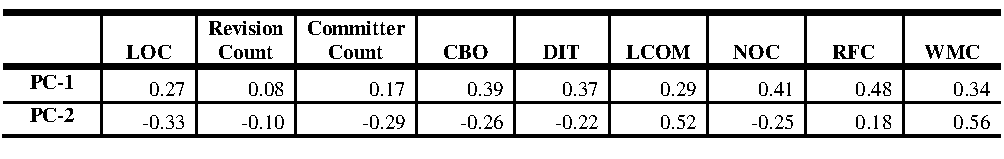
\includegraphics[width=1.0\textwidth]{TeamSizePCA.pdf}
 \label{tab:TeamSizePCA}
\end{tabular}
\end{table}

Figure ~\ref{fig:TeamSizeScatter} shows a depiction of the team size sample scattered across these two principal components. No distinct clusters immediately emerge from this, but through this process it is possible to select two projects which are visually distant from one another for further study.

\begin{figure}[htbp!] 
\centering    
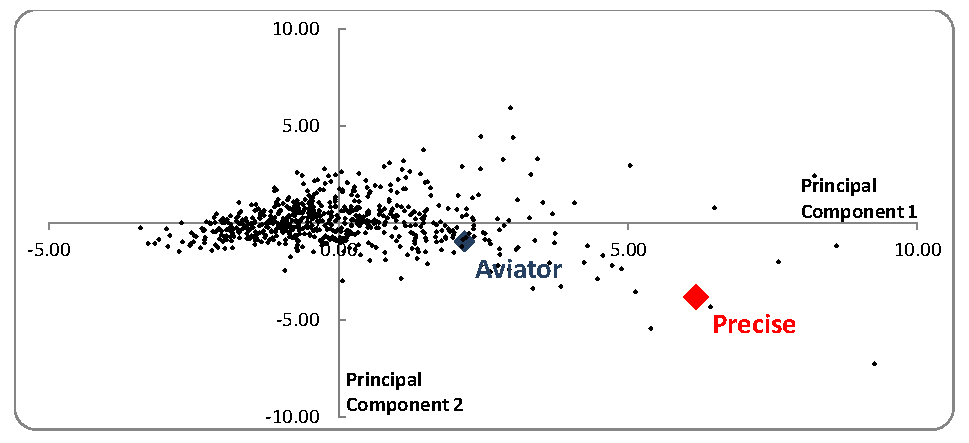
\includegraphics[width=1.0\textwidth]{TeamSizeScatter.pdf}
\caption{A visualisation of the team size sample scattered across the two principal components. The selection of Aviator and Precise for further study.}
\label{fig:TeamSizeScatter}
\end{figure}

Aviator and Precise are two projects that exhibit metric values that, relative to each other, are consistent with the wider forge trends for the given team sizes: one and five committers respectively. Aviator is located on the edge of the main cluster while Precise appears very much as an outlier - likely owing to its higher than mean LOC. Figure ~\ref{fig:TeamSizesResultsCompare} shows a comparison of the metric profiles between these two projects plotted against revision counts. Aviator is an expression engine that dynamically compiles expressions into Java byte-code and delivers them to a running JVM. It is a single committer project with the full codebase in Java and no graphical user interface. The project comprises 233 Java class files. The committer is currently a prolific contributor to open-source projects with an active public GitHub profile. The Aviator project represented one of his early efforts started after he had accumulated roughly 2 years of development experience. 

Precise is a requirements modelling and tracking tool designed to plug into the Eclipse IDE, with no dedicated user-interface as such. The project codebase comprises 524 Java class files alongside some modelling artefacts. Four distinct committers contributed to this project over a period of two years with the activity levels shown in ~\ref{fig:PreciseCommitterAnalysis}. It is notable that one committer contributes very little commits to the project while two committers contribute the majority of commits and unique files. The definition of team size within this research does not distinguish between the activity levels of committers in assigning a value to this measure. However, the final chapter of this thesis does consider avenues of future work to assess the impact to regression models by distinguishing between core and peripheral committers in the calculation of team size.

\subsection{Project Comparison}
Figure ~\ref{fig:TeamSizesResultsCompare} shows a comparison of the metric profiles between two projects plotted against revision counts. As previously, metric values are bucketed by revision count and averaged. It is notable that the observations for Precise are higher than those for Aviator for those metrics most affected by team size according to the linear regressions; CBO, DIT and LCOM. CBO and LCOM trend up with revisions, as expected given the positive coefficient estimates of the linear models. DIT does not exhibit a consistent trend against revision counts which is consistent with the earlier results which assigned a coefficient of zero to revision counts ($\beta_R$). 

\begin{figure}[htbp!] 
\centering    
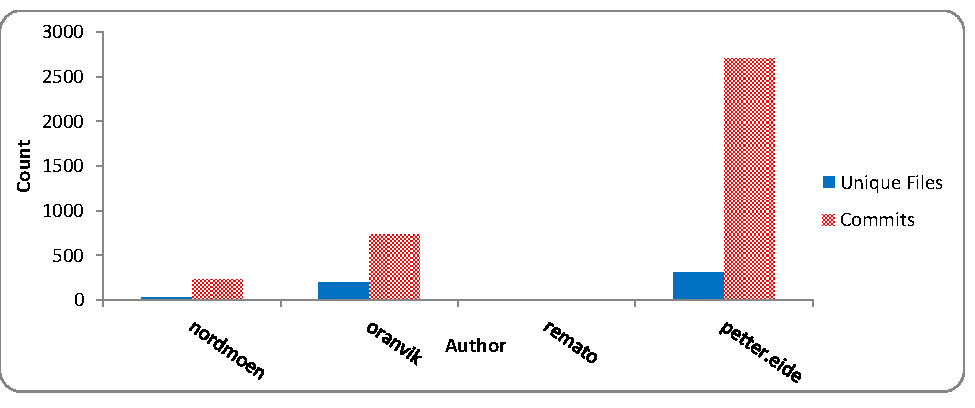
\includegraphics[width=1.0\textwidth]{PreciseCommitterAnalysis.pdf}
\caption{Committer behaviour analysis for the Precise project.}
\label{fig:PreciseCommitterAnalysis}
\end{figure}

\begin{figure}[htbp!] 
\centering    
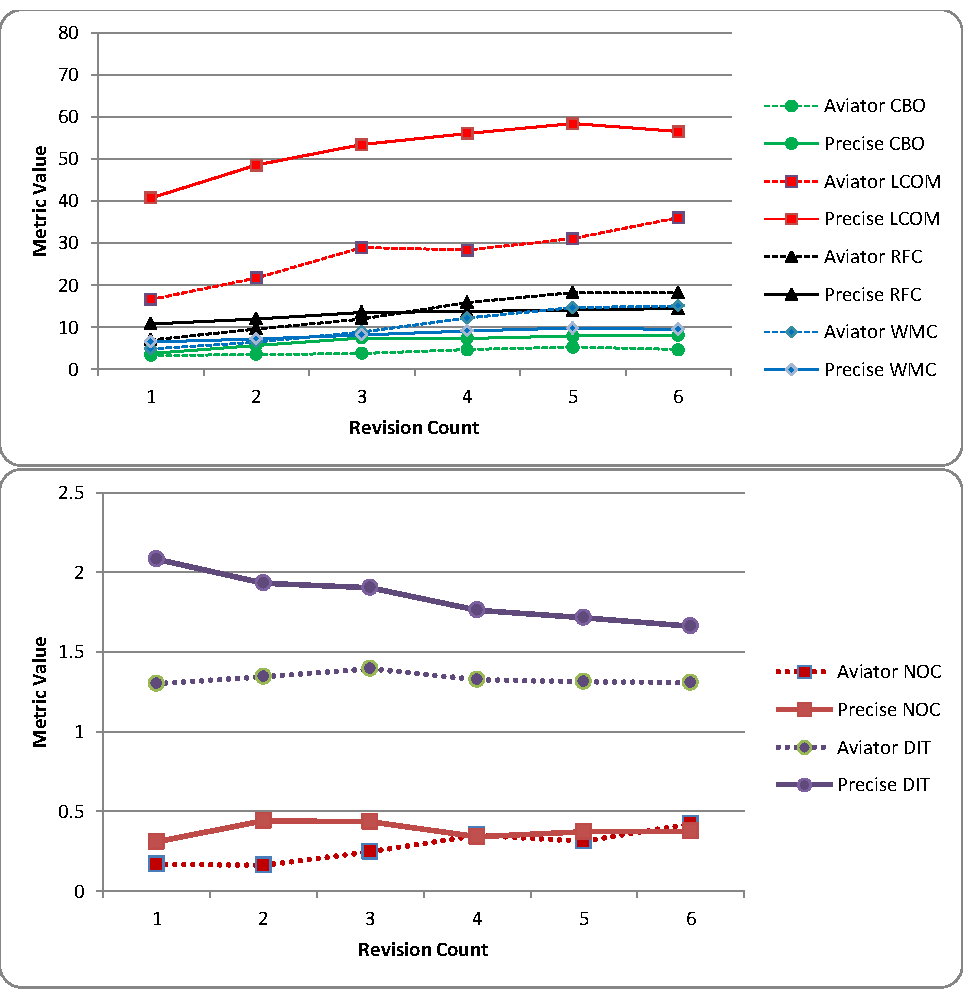
\includegraphics[width=1.0\textwidth]{TeamSizesResultsCompare.pdf}
\caption{Key structural attributes for the single contributor Aviator project compared against multi-contributor project Precise.}
\label{fig:TeamSizesResultsCompare}
\end{figure}

Within the Precise project there is some obvious fragmentation which can be observed through a fairly dis-organised source folder and package structure. Many classes are too large with 28 classes over 250 lines long, with code violating the 'single responsibility' principle which dictates that a class should do one thing and do it well. Failure to adhere to this leads to a lack of cohesion as member variables are rarely relevant to all methods in a fragmented class. Similarly a large number of methods would lead to a high values for WMC and CBO which are capture structural complexity and modularity respectively. To illustrate, Figure ~\ref{fig:BadCodeExample} shows a snippet of code from one of the most complex classes which contains 635 lines and 35 methods, most of which contain complex functionality. In one method there are seven nested conditional blocks, indicative of inordinate structural complexity and poor modularity. The revision history of this particular class shows that it had three distinct committers and had a high degree of structural complexity from the initial creation which steadily increased over subsequent revisions.
 
Precise has a significantly larger and more fragmented codebase than Aviator which appears to lead to fairly large class files with multiple responsibilities and points of coupling with other classes. By way of example, the ASMCodeGenerator class has responsibilities for code generation, arithmetic operations and maintaining complex collection structures indicating poor cohesion. Furthermore, as illustrated in ~\ref{fig:BadCouplingExample}, it directly coupled to multiple concrete implementations within the codebase, albeit mostly functionally oriented to code generation.  It is reasonable to postulate that a lack of effective coordination between committers on the Precise project lead, at least in part, to this fragmentation. This is a vicious cycle as poor structural attributes leads to further degradation as the codebase becomes more difficult to navigate and the demands for effective coordination between committers become unwieldly. All evidence is that the Precise project never made it to a fully-fledged release and ultimately failed as a project. Meanwhile Aviator continued to remain under active development after GoogleCode was decommissioned, migrating to GitHub and registering numerous releases.

\begin{figure}[htbp!] 
\centering    
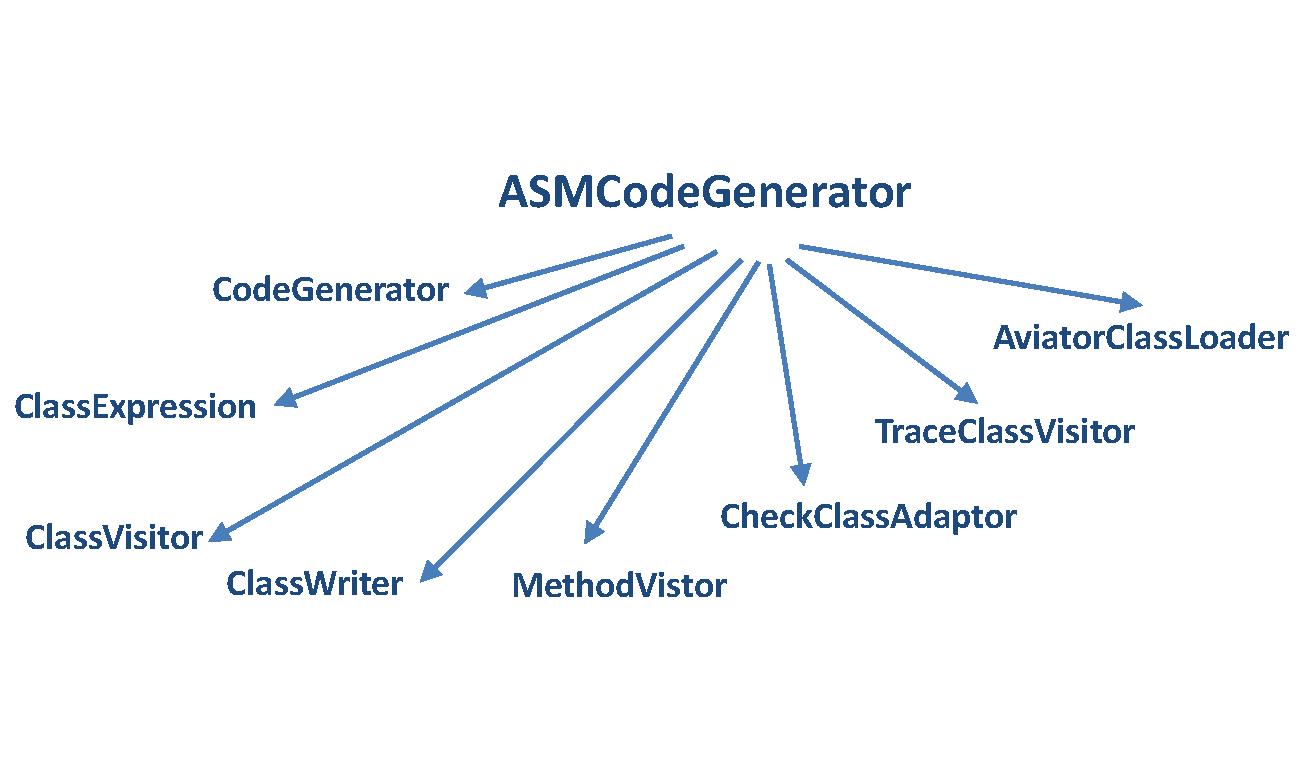
\includegraphics[width=1.0\textwidth]{BadCouplingExample.pdf}
\caption{A depiction of the external dependencies to which the ASMCodeGenerator class is coupled.}
\label{fig:BadCouplingExample}
\end{figure}

\begin{figure}[htbp!] 
\centering    
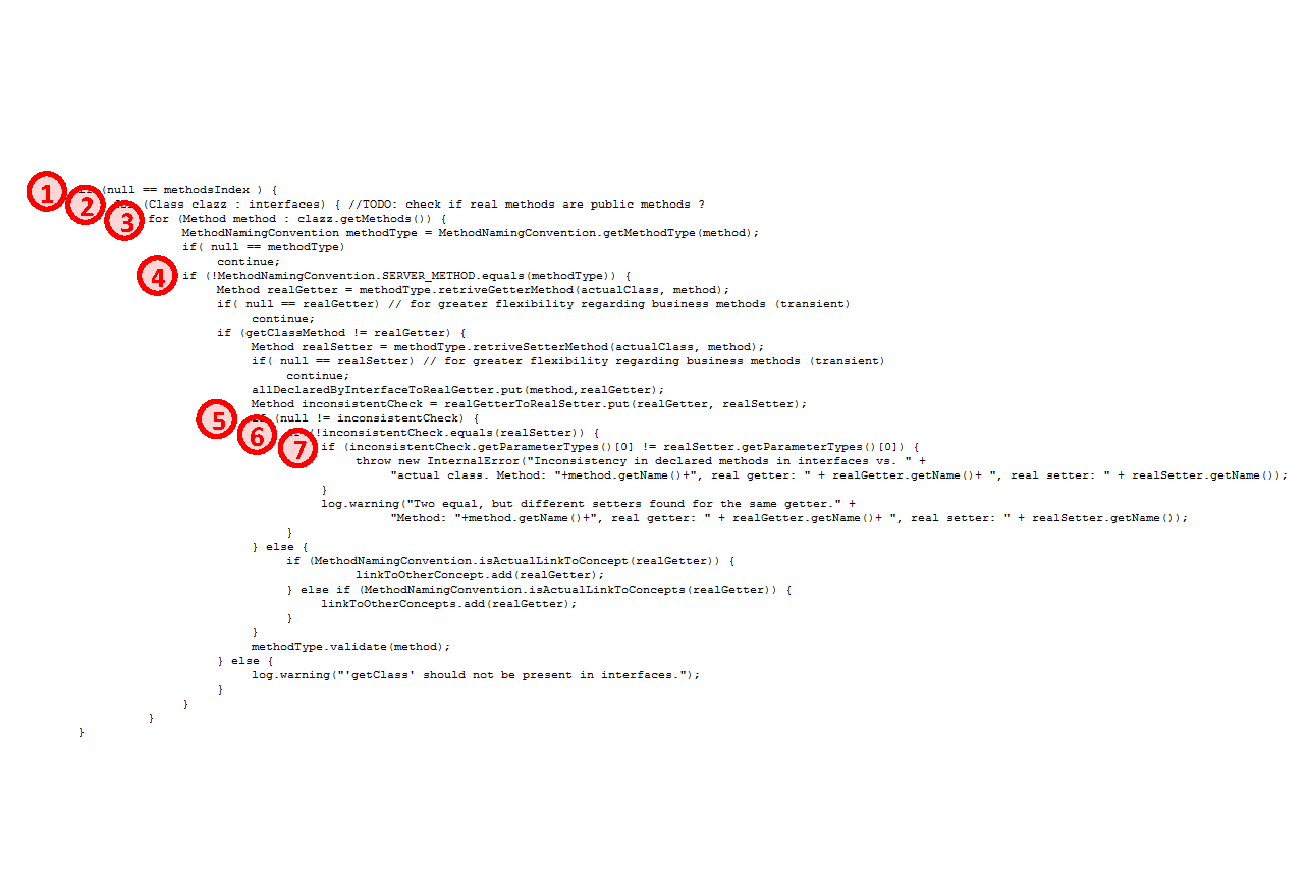
\includegraphics[width=1.0\textwidth]{BadCodeExample.pdf}
\caption{A code snippet from the DomainProxyInvocationHandler class within the Precise project. The nested iterative blocks are numerically labelled.}
\label{fig:BadCodeExample}
\end{figure}

\begin{table}
\centering 
\captionof{table}{The intercepts and residuals for the Precise and Aviator projects.}
\begin{tabular}
 \centering 
 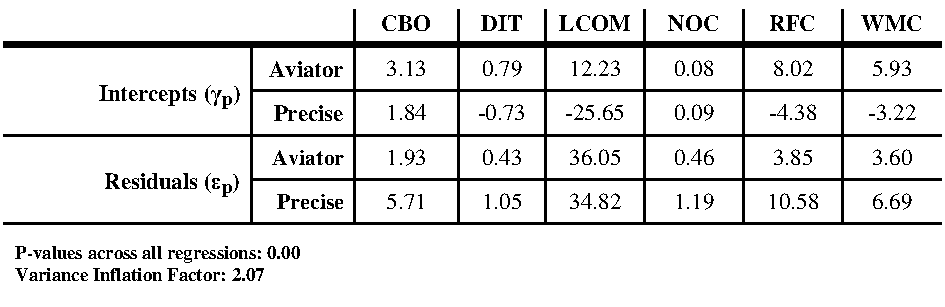
\includegraphics[width=1.0\textwidth]{RandomInterceptsLinearRegressionSelectedProjects.pdf}
 \label{tab:RandomInterceptsLinearRegressionSelectedProjects}
\end{tabular}
\end{table}

Table ~\ref{tab:TeamSizePCA} shows the intercept and residual values for the Precise and Aviator projects from the LMM regression in the previous section. The residual values of Aviator and Precise are consistent with their respective positions in the scatter plot. Precise, as an outlier in the scatter plot, could reasonably be expected to have a regression line that is compromised by the nature of the majority of the projects in the sample that make up the main cluster. This is reflected in higher residual values relative to the Aviator project. Conversely, the intercept values for the Precise project are significantly higher than Aviator. This is a result of the greater distance to the y-axis when extrapolating regression lines to achieve intercepts for projects with a higher team size. Given that projects with larger team sizes will have 'further to travel' in order to intercept with the y-axis, and that all projects will  have share a single gradient (the coefficient estimate) for a given metric regression, it is logical that those projects with a higher team sizes are likely to have lower (or even negative) intercepts. These observations help illustrate the strength of LMMs over OLS regression models within this context.

\section{Summary of Analysis} %Section - 4.7
To recap the analysis in this chapter, at the outset there was basic exploratory data analysis revealing underlying trends around committer behaviour and the nature of a commit as well as the distribution and correlations between the key variables in the data set. The analysis then moved on to tackling the first research question (RQ1) to establish if there was a relationship, at a forge level, between team size (the independent factor) and CK metrics (dependent factor). Then, following in the approach of the prior literature, there was a study of two factors for potential confounding impact, code size and revisions. It was determined that the former was not a confounding variable but the latter is. Revisions were then controlled for as a part of the next phase of analysis. The analysis to this point was achieved by taking observations from across projects and grouping them by team size and later by revisions, but always out of the context of the project from which they came. The latter section used the mixed models approach to linear regression to retain the project-specific idiosyncratic element to the data, re-evaluating the coefficient estimates and generate lower residuals. Finally the forge sample was visualised on a scatterplot, using PCA for dimensionality reduction, enabling the selection of two distinct projects for further qualitative and quantitative study. This helped shed light on the code-level features that drove the relationships reported by the linear models.

The results showed that projects developed by larger team sizes exhibited an increase in coupling (reflected by larger CBO values), an increase in inheritance complexity (reflected by higher DIT values) and a decrease in cohesion (reflected by larger LCOM values). This is a rejection of the null hypothesis H0,1 which anticipated no impact to any of the structural attributes of the software. Similarly, this leads us to accepting the alternate hypothesis H1,1.1, the basis of which was that prior research had linked larger teams to greater fault-proneness and, in the absence of further data, it was reasonable to hypothesise that maintainability and fault-proneness could be negatively correlated. There is consistency between the results of this team size analysis and the research of Nagappan et al. \citep{nagappan2008influence} who linked larger team sizes with increased fault-proneness given that Basili et al. had confirmed that CBO and DIT is highly correlated with fault-proneness \citep{basili1996validation}; this research having also observed higher CBO and DIT values from larger team sizes.

Referring to Table 2.5 (the survey of research correlating CK metrics to the sub-attributes of maintainability), inferences can be drawn from the observed structural trends against the impact on the maintainability of the software. Bruntink et al. had observed that DIT was negatively correlated with the testability while Badri et al. noted the same relationship between LCOM and testability \citep{bruntink2006empirical, badri2011empirical}. Harrison et al. found that LCOM was negatively correlated with changeability and Elish and Rine found that all CK metrics were negatively correlated with stability \citep{harrison1998investigation, elish2003investigation}.

Based on this prior research it can be deduced from the results of this chapter that the increased coupling, inheritance complexity and decreased cohesion of software associated with larger team sizes - represented by the higher values of CBO, DIT and LCOM respectively - result in degraded levels of the maintainability sub-attributes of testability, changeability and testability. This is an acceptance of alternate hypothesis H1,1.2 and is depicted in Figure ~\ref{fig:ResultOverview}.

\begin{figure}[htbp!] 
\centering    
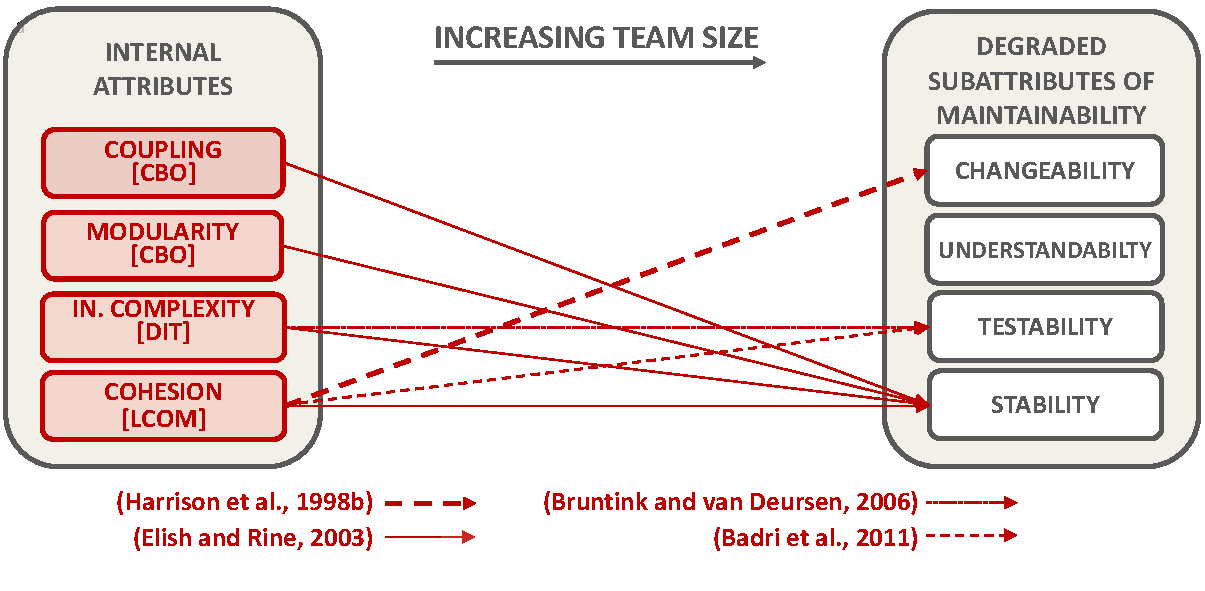
\includegraphics[width=1.0\textwidth]{ResultOverview.pdf}
\caption[The impact of internal attributes on the maintainability of software.]{The impact of structural attributes on the maintainability of software. Coupling, cohesion and modularity and inheritance complexity all trend in a direction that indicates an attendant degradation in testability and stability and changeability.}
\label{fig:ResultOverview}
\end{figure} 
  
 \section{Chapter Review} %Section - 4.5
This chapter studied the relationship between development team size and the CK metrics of the produced software. This was done by first sampling the broader GoogleCode forge followed by exploratory data analysis studying committer behaviour and comparing the sample to the broader forge. Simple linear models were produced and the confounding factor of revision counts was identified. The multivariate analysis introduced revision counts into the linear model and, through studying individual projects in detail, the nature of the linear relationship was established.

The next chapter uses a similar approach to study the impact of team stability on the structural attributes of software. A distinction will be drawn between the team stability that is developed through the commit history of a project and the team stability that accrues across multiple projects.